\documentclass[sigplan,10pt,review,anonymous]{acmart}
\settopmatter{printfolios=true,printccs=false,printacmref=false}

\acmConference[Submitted to PLDI'18]{ACM SIGPLAN Conference on Programming Language Design and Implementation}{June 18--22, 2018}{Philadelphia, PA, USA}

\acmYear{2018}
\acmISBN{} % \acmISBN{978-x-xxxx-xxxx-x/YY/MM}
\acmDOI{} % \acmDOI{10.1145/nnnnnnn.nnnnnnn}
\startPage{1}
\setcopyright{none}

%% Some recommended packages.
%\usepackage{booktabs}   %% For formal tables: http://ctan.org/pkg/booktabs
\usepackage{subcaption} %% For complex figures with subfigures/subcaptions http://ctan.org/pkg/subcaption
%\usepackage[normalem]{ulem}
%\usepackage{float}
\usepackage{soul}
\usepackage{amssymb}
\usepackage{amsmath}
\usepackage{algorithm} % environment for the algorithm code (like figure and table)
\usepackage{algorithmicx} % write the pseudo code
\usepackage[noend]{algpseudocode} % layout of the pseudo code
\usepackage{tikz} % needed for: tikz pics
\usepackage{xcolor}
\usepackage{xspace}
\usepackage{listings}

%\usepackage[keeplastbox]{flushend} %Brandon: this broke the build for me
%Added for sub-float package from jpaper.cls - will check later
%\RequirePackage[font={normalsize,sf,bf}]{caption}
%\RequirePackage[position=bottom]{subfig}
%\captionsetup[table]{aboveskip=0.5em, belowskip=0.5em}
%\captionsetup[figure]{aboveskip=0.5em, belowskip=0em}
\captionsetup[subfloat]{font={small,sf}}

\hypersetup{colorlinks=false,linkcolor=blue,urlcolor=blue}

\newlength{\sectionbelowskip}
\newlength{\sectionaboveskip}
\newlength{\subsectionbelowskip}
\newlength{\subsectionaboveskip}
\newlength{\paragraphaboveskip}

% Defaults in sigplanconf (note that horizontal space after \paragraph heading will be different):
%\setlength{\sectionbelowskip}{4pt}
%\setlength{\sectionaboveskip}{10pt plus 3pt minus 2pt}
%\setlength{\subsectionbelowskip}{4pt}
%\setlength{\subsectionaboveskip}{8pt plus 2pt minus 2pt}
%\setlength{\paragraphaboveskip}{6pt plus 2pt minus 2pt}

% Slightly tighter than defaults:
% \setlength{\sectionbelowskip}{3pt}
% \setlength{\sectionaboveskip}{6pt plus 2pt minus 2pt}
% \setlength{\subsectionbelowskip}{2pt}
% \setlength{\subsectionaboveskip}{4pt plus 1pt minus 1pt}
% \setlength{\paragraphaboveskip}{2pt plus 1pt minus 1pt}

% Tighter than defaults:
\setlength{\sectionbelowskip}{1pt}
\setlength{\sectionaboveskip}{5pt plus 1.5pt minus 1.5pt}
\setlength{\subsectionbelowskip}{1pt}
\setlength{\subsectionaboveskip}{3pt plus 1pt minus 1pt}
\setlength{\paragraphaboveskip}{1pt plus 1pt minus 1pt}

\newcommand{\TODO}[1]{{\bf \em \textcolor{red}{TODO: #1}\xspace}}
\newcommand{\todo}[2]{\textcolor{red}{$\bullet$ \textbf{Task:} #1; \textbf{Responsible:} #2}}
\newcommand{\add}[1]{\textcolor{blue}{#1}}
\newcommand{\remove}[1]{\textcolor{red}{\st{#1}}}
\newcommand{\replace}[2]{\remove{#1} \add{#2}}

\newcommand{\transition}{{\tt next\_task}\xspace}
\newcommand{\sys}{Coala\xspace}
\newcommand{\sysmed}{\sys: Adaptive Task Coalescing $\ldots$}
\newcommand{\sysfull}{\sys: Adaptive Task Coalescing for Intermittent Computing on Energy-harvesting Devices}
%newcommand{\sysfull}{\sys: Efficient Task-based Intermittent Computing with Adaptive Task Coalescing and Memory Virtualization} %Old title

\begin{document}

\title[\sysmed]{\sysfull}

%Note: order of authors placed randomly

%\author{Kiwan Maeng}
%\authornote{}
%\orcid{}
%\affiliation{%
%	\institution{Carnegie Mellon University}
%	\streetaddress{4720 Forbes Avenue}
%   \city{Pittsburgh} 
%	\state{PA} 
%	\postcode{15213}
%}
%\email{kmaeng@andrew.cmu.edu}

%\author{Alexei Colin}
%\authornote{}
%\orcid{}
%\affiliation{%
%	\institution{Carnegie Mellon University}
%	\streetaddress{4720 Forbes Avenue}
%	\city{Pittsburgh} 
%	\state{PA} 
%	\postcode{15213}
%}
%\email{acolin@andrew.cmu.edu}

%\author{Brandon Lucia}
%\authornote{}
%\orcid{}
%\affiliation{%
%	\institution{Carnegie Mellon University}
%	\streetaddress{4720 Forbes Avenue}
%	\city{Pittsburgh} 
%	\state{PA} 
%	\postcode{15213}
%}
%\email{blucia@andrew.cmu.edu}

%\author{Amjad Yousef Majid}
%\authornote{}
%\orcid{}
%\affiliation{%
%	\institution{Delft University of Technology}
%	\streetaddress{Mekelweg 4}
%	\city{Delft, The Netherlands} 
%	\state{Zuid Holland} 
%	\postcode{2628\,CD}
%}
%\email{a.y.majid@tudelft.nl}

%\author{Kas{\i}m Sinan Y{\i}ld{\i}r{\i}m}
%\authornote{}
%\orcid{}
%\affiliation{%
%	\institution{Delft University of Technology}
%	\streetaddress{Mekelweg 4}
%	\city{Delft, The Netherlands} 
%	\state{Zuid Holland} 
%	\postcode{2628\,CD}
%}
%\email{k.s.yildirim@tudelft.nl}

%\author{Przemys{\l}aw Pawe{\l}czak}
%\authornote{}
%\orcid{}
%\affiliation{%
%	\institution{Delft University of Technology}
%	\streetaddress{Mekelweg 4}
%	\city{Delft, The Netherlands} 
%	\state{Zuid Holland} 
%	\postcode{2628\,CD}
%}
%\email{p.pawelczak@tudelft.nl}

%\renewcommand{\shortauthors}{A. Y. Majid et al.}

\begin{abstract}
	
Computation consistency on intermittently-powered devices can be ensured by: (i) checkpointing, where the volatile state of a program is frequently saved to non-volatile memory, or (ii) via tasks, where a programmer splits the code into small idempotent sections. Results so far suggest that a task-based approach performs better than checkpointing. However, existing tasks-based approaches do not adapt to changing energy levels and storage. This makes the code inefficient (when executed on a larger energy buffer than intended) or can potentially completely disable the program (in the opposite case). Therefore, we present \sys: a task-based execution runtime, enabling code portability by means of a new concept of task coalescing. If a code is written for a very small energy buffer, \sys is able to dynamically coalesce these tasks and constructs a bigger (virtual) task to improve execution times. \todo{Provide concrete numbers for improvement}{Amjad} \todo{Provide concrete numbers for checkpointing improvement}{Amjad}

\end{abstract}

% The code below should be generated by the tool at 
%http://dl.acm.org/ccs.cfm Please copy and paste the code instead of the 
%example below. 

%\begin{CCSXML}
%	<ccs2012>
%	<concept>
%	<concept_id>10010520.10010553.10010562.10010564</concept_id>
%	<concept_desc>Computer systems organization~Embedded 
%	software</concept_desc>
%	<concept_significance>500</concept_significance>
%	</concept>
%	<concept>
%	<concept_id>10010520.10010575.10010578</concept_id>
%	<concept_desc>Computer systems organization~Availability</concept_desc>
%	<concept_significance>300</concept_significance>
%	</concept>
%	<concept>
%	<concept_id>10011007.10010940.10010941.10010949.10010957.10010688</concept_id>
%	<concept_desc>Software and its engineering~Scheduling</concept_desc>
%	<concept_significance>300</concept_significance>
%	</concept>
%	<concept>
%	<concept_id>10011007.10010940.10010941.10010949.10010965</concept_id>
%	<concept_desc>Software and its engineering~Communications 
%	management</concept_desc>
%	<concept_significance>300</concept_significance>
%	</concept>
%	<concept>
%	<concept_id>10011007.10010940.10010971.10010564</concept_id>
%	<concept_desc>Software and its engineering~Embedded 
%	software</concept_desc>
%	<concept_significance>300</concept_significance>
%	</concept>
%	</ccs2012>
%\end{CCSXML}

%\ccsdesc[500]{Computer systems organization~Embedded software}
%\ccsdesc[300]{Computer systems organization~Availability}
%\ccsdesc[300]{Software and its engineering~Scheduling}
%\ccsdesc[300]{Software and its engineering~Communications management}
%\ccsdesc[300]{Software and its engineering~Embedded software}

%\keywords{Energy harvesting, transient operation, operating system}

\maketitle

\section{Introduction}
\label{sec:intro}

%%%%%%%%%%%%%%%%%%%%%% IMPORTANT INFO %%%%%%%%%%%%%%%%%%%%%%%%%%%%%%
% SRAM read/write latency is in the order of 8ns 		 [ Intermittent computation without hardware support of programmer intervention]
% FRAM read/write latency is in the orfer of 60ns/100ns  [Texas Instrument MSP430FR573x DataSheet]
%%%%%%%%%%%%%%%%%%%%%%%%%%%%%


Advances in processor efficiency along with the development of
energy-harvesting systems has created a new category of devices that require
neither a battery nor a tethered power
supply~\citep{prasad_comst_2014,lucia_snapl_2017,soyata_csm_2016}. These
devices operate using ambient energy, such as radio frequency
transmissions~\citep{rf_powered_computing_gollakota_2014},
light~\citep{margolies_infocom_2016,margolies_tosn_2016}, and
vibration~\citep{gorlatova_sigmetrics_2014}. Incorporating compute, storage,
sensing, and communication hardware~\citep{wisp5,moo,capybara}, such devices are a
promising technology for use in the Internet of Things~\citep{ku_cst_2016},
in-body~\citep{nadeau_naturebio_2017} and
on-body~\citep{bandodkar_electroanalysis_2015} medical systems, and
energy-harvesting nano-satellites~\citep{kicksat,capybara}.

Energy-harvesting devices create unique challenges because they operate {\em
intermittently} when energy is
available~\citep{hicks_isca_2017,lucia_snapl_2017}. An energy-harvesting device
buffers energy in a small storage capacitor~\citep{gorlatova_tmc_2013,gunduz_commag_2014} and operates when a
threshold amount of energy has accumulated. Harvestable energy sources are low-power (e.g., nW to $\mu$W) compared to a platform's operating
power level (hundreds of $\mu$W to mW). A device operates briefly until it depletes its buffered energy, after which, the device shuts
down and recharges to operate again later---corresponds to {\em intermittent execution model}~\citep{dino,lucia_snapl_2017} composed of
operation-power failure-restart cycles. As an example, recharge times may be
tens of seconds in radio frequency powered medical device~\cite[Fig.
3c]{nadeau_naturebio_2017}.  The recharge and discharge time---which corresponds to the device's inactive and active time---varies with the energy buffering capacitor's~\cite{capybara} and some devices fail and restart operating $\approx$10 to
$\approx$100 times per second~\citep{tan_infocom_2016,mementos,nvp}.  

\begin{wrapfigure}{t!}{0.5\textwidth}
    \centering
    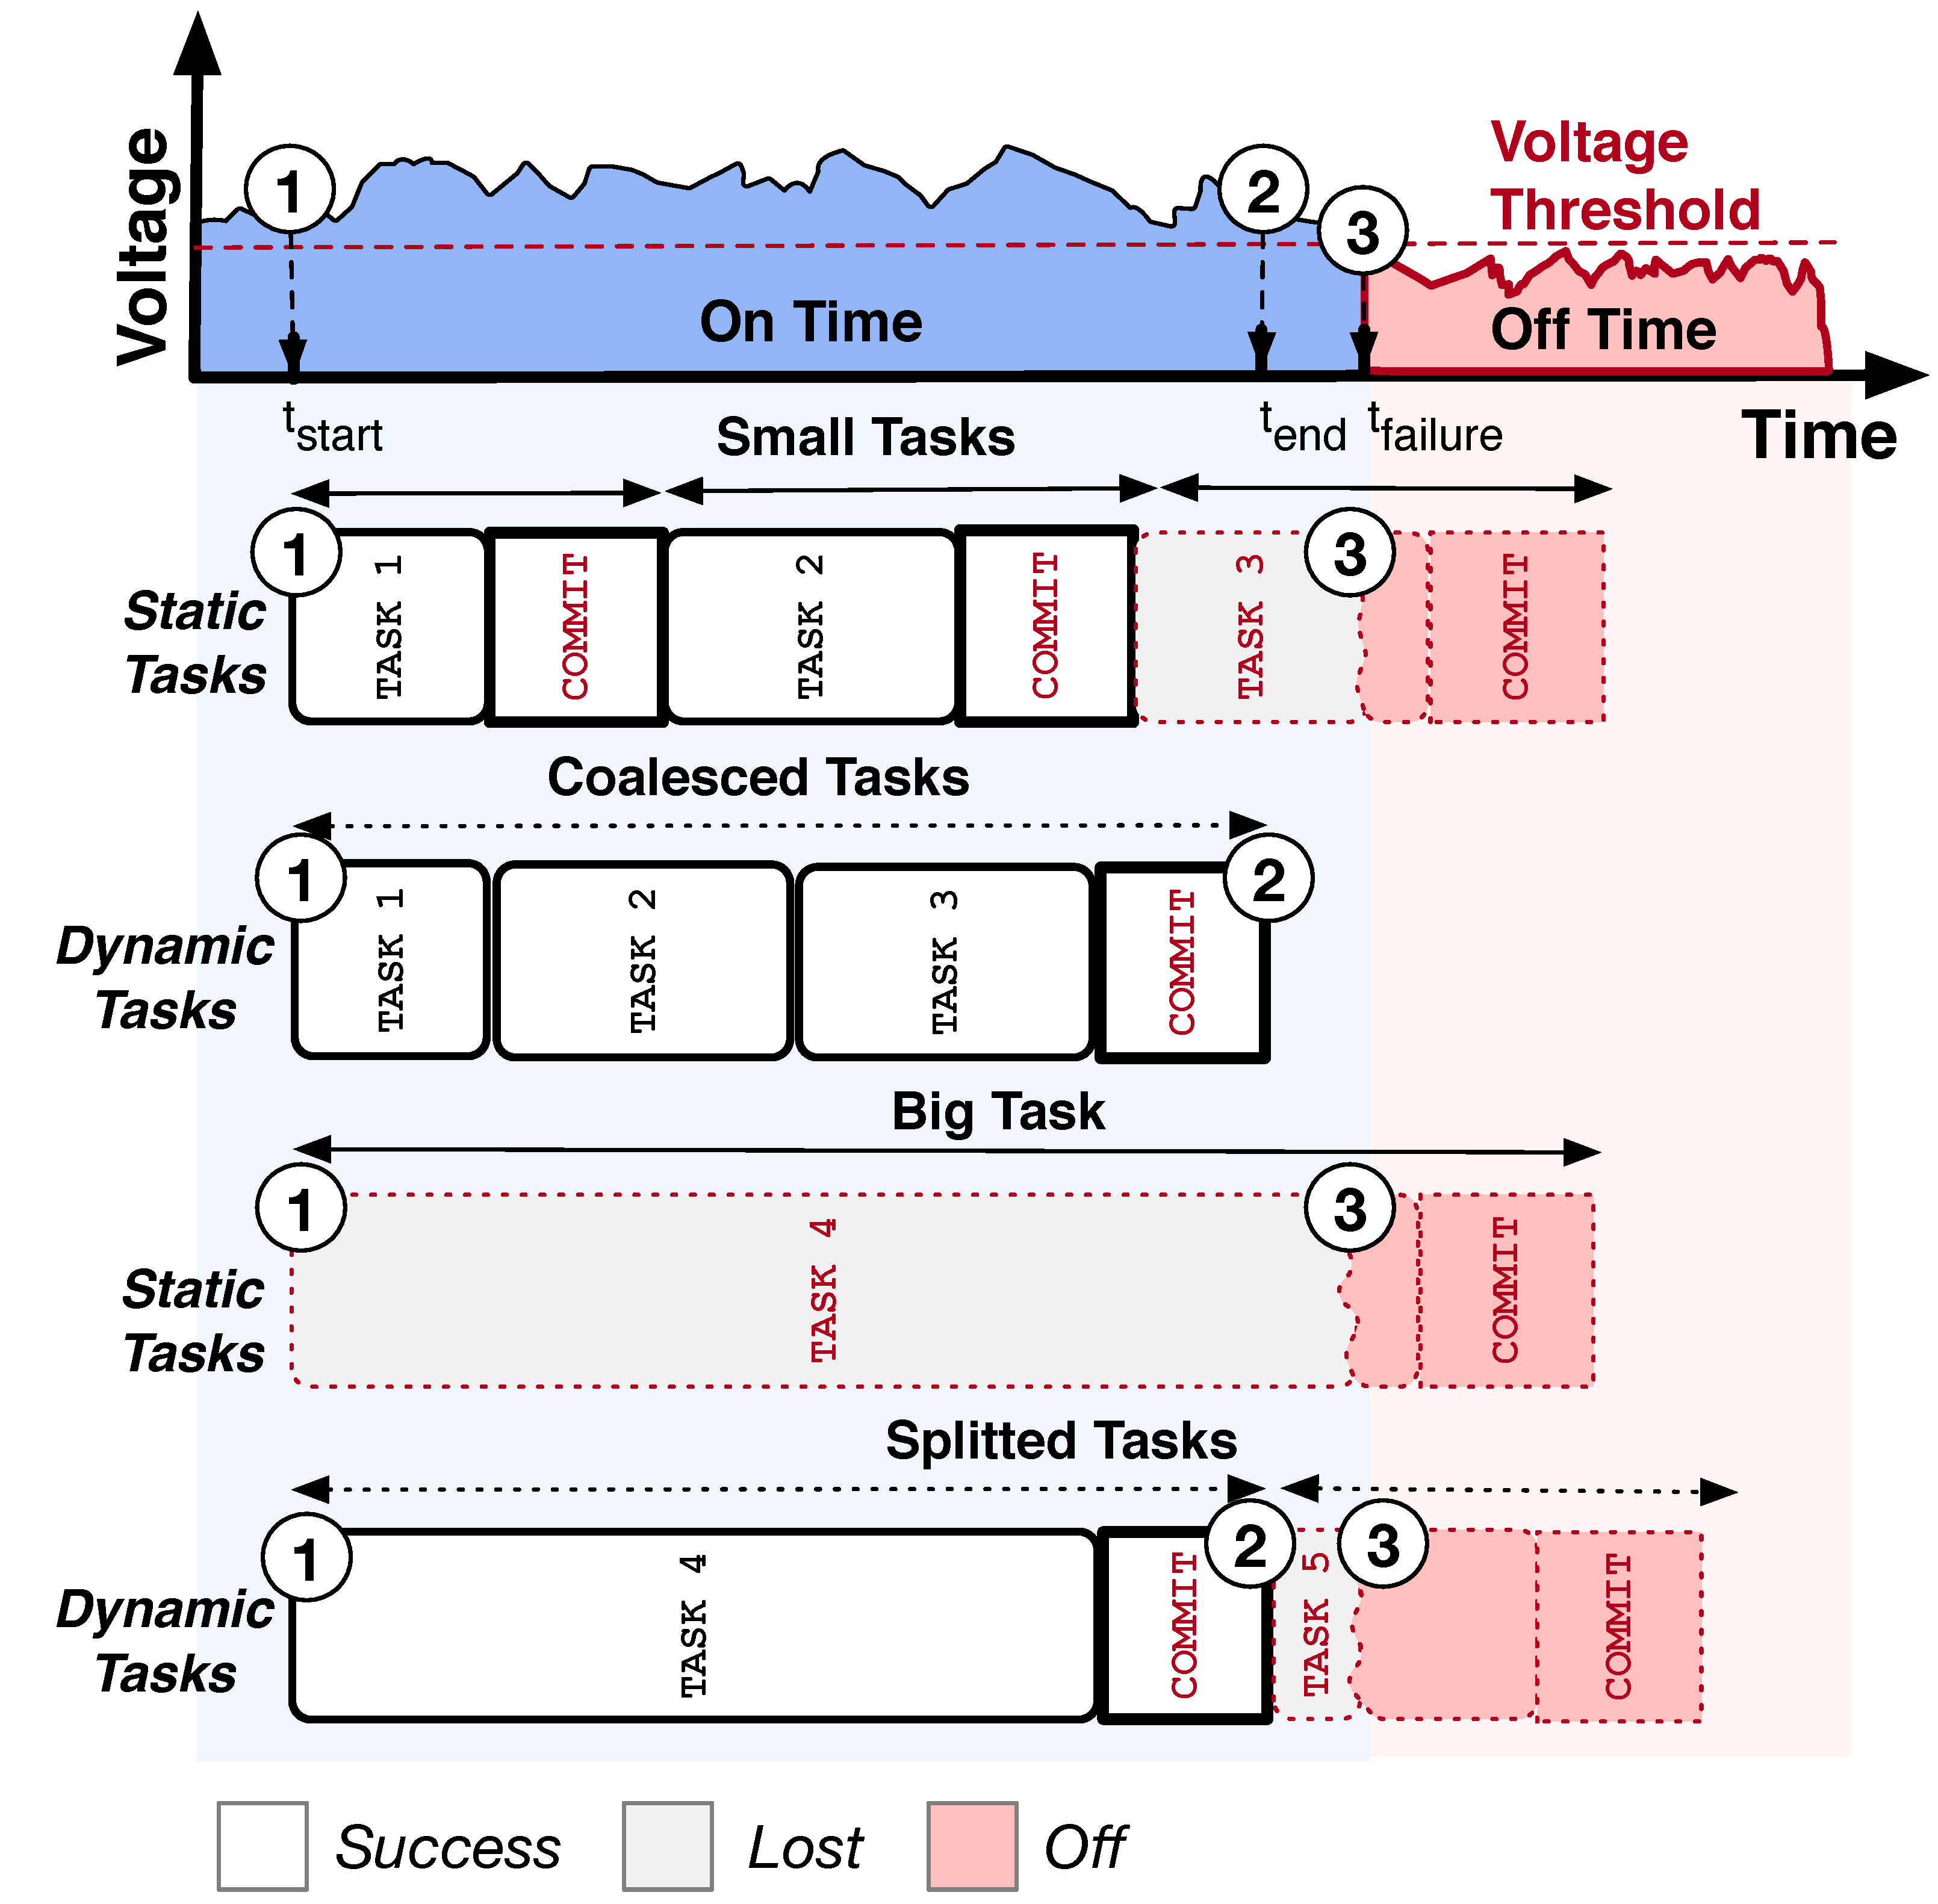
\includegraphics[width=0.5\textwidth]{figures/graffle/intro-figure.pdf}
    \caption{Task coalescing at runtime reduces time and energy overhead in task-based intermittent programming models by performing fewer commits. On the other hand, task splitting reduces wasted computation and enables termination for bigger tasks.}
    \label{fig:coalesce}
\end{wrapfigure}

\textbf{Data Consistency in Intermittent Computing.}  
%Software in an energy-harvesting system operates according to the {\em intermittent execution model}~\citep{dino,lucia_snapl_2017}, which corresponds to the operation-failure-restart cycles of an energy-harvesting device. In an intermittent software execution, an {\em operating period} proceeds for anarbitrary duration (dictated by energy availability) before being interruptedby a {\em failure period}. In a failure period, 
Upon power failures, a device loses the volatile
state in its registers, stack, SRAM, and retains the state of any non-volatile
memory, such as FRAM or Flash. While capturing periodic
checkpoints~\citep{mementos,quickrecall} and sleep
scheduling~\citep{dewdrop,hibernus,hibernusplusplus} help preserve execution
progress, failures can leave non-volatile state incorrectly, partially updated,
and may leave checkpointed volatile state inconsistent with non-volatile state.
These inconsistencies cause intermittent execution to deviate from
continuously-powered behavior, often leading to an unrecoverable
application failure~\citep{dino,edb}. Prior work developed two main approaches to dealing with data inconsistency for
intermittently-powered devices: (i) \emph{software-based programming and
execution models}~\citep{dino,ratchet,chain,alpaca} and (ii)
\emph{hardware-based computer architecture
support}~\citep{hicks_isca_2017,idetic,nvp}.  Complex architectural changes are
expensive to design, verify, and manufacture.  New architectures are also
inapplicable to existing systems~\citep{hicks_isca_2017,nvp}. Software
approaches are simpler and applicable to existing devices today, but prior
software approaches have a number of limitations that are the focus of the work
in this paper.  A key limitation of prior software approaches that we address in this paper is the {\em inflexibility} of a program statically decomposed into tasks. 

\textbf{Task Decomposition of Intermittent Programs.} {\em
Task-based} programming and execution models require a
programmer~\citep{alpaca,chain} or a compiler~\cite{baghsorkhi_cgo_2018} to
statically decompose a program into a collection of {\em tasks}.  A task can
include arbitrary computation that should be executed despite arbitrarily-timed power failures.
%and these existing systems guarantee that each
%tasks executes {\em atomically}, despite arbitrarily-timed power failures.  
%
The programmer explicitly expresses task-to-task control flow, or the compiler
converts existing program control-flow into task-to-task control flow to sequence 
the tasks that it defines.
%
Figure~\ref{fig:coalesce} (top) illustrates how a program's tasks execute and
shows how tasks can impose a run-time overhead. 
%
At each task transition, the system incurs an overhead to track and atomically
\emph{commit} modifications to the non-volatile memory, to maintain consistency of
program state~\citep{chain,alpaca}.  
%
The more task transitions a program requires, the more commit overhead is incurred by the system at run-time.

A savvy programmer may thus create very large tasks in an attempt to minimize
overhead by minimizing the number of task transitions.  However, a very large
task may require more energy to complete than a device's fixed hardware energy
buffer can hold.  Such a large task fails to completely execute assuming only
buffered energy is available (i.e., assuming the worst case).  While some
environments may have sufficient harvestable energy to replenish a device's
capacitor during operation, prolonging the execution period and enabling the
task to complete, assuming cooperation from the physical environment to avoid
non-termination is a risky programming proposition.  To eliminate this risk,
existing systems require the programmer or compiler to decompose a  program
into small tasks, all of which complete using only buffered energy.  These
constraints on task sizing leave an unsatisfying dilemma: large, efficient
tasks that risk non-termination, or small tasks that are guaranteed to
complete, but incur a high task transition and commit overhead.  In this work,
we propose a third way, using a novel technique called {\em adaptive execution by dynamic task
coalescing/splitting} that efficiently executes small tasks, avoiding unnecessary overheads while avoiding the risk of non-termination.

%A key challenge is that the length of a software
%task's execution is \emph{limited by the fixed total amount of energy} that a
%device can buffer in hardware. A task's code is static, but the duration of its
%execution may be input-dependent and is difficult to predict. To illustrate
%this, we refer to Figure~\ref{fig:1} showing the execution time of two
%applications (the same application X, but divided into X and Y tasks as
%in~\citep{chain}) running on RFID antenna-powered Computational
%RFID~\citep{wisp,rf_powered_computing_gollakota_2014} at two device-to-antenna
%distances (near---stable energy supply/far---high energy intermittency). At
%short distance: execution will takes too long caused by runtime cost of
%marshalling excessively small tasks. At far distance: program \emph{might never
%execute} if task execution consumes more energy than the system can buffer.
%This calls for at-runtime adaptive task division of any transiently-powered
%application---namely \emph{task virtualization}.

In this work, we introduce a new system called \sys, which executes a task-based
intermittent program by dynamically coalescing its tasks.
\sys accepts any static decomposition (i.e., from the programmer or from a compiler) 
and coalesces its tasks at runtime. Two consecutive, coalesced tasks execute  
with no commit or task transition overhead between them, instead performing
task-end commit actions at the end second task only.
%
When there is sufficient energy to execute both tasks, two distinct, small
tasks are effectively executed as a single large task, preserving the atomicity
of both.  If power fails during a coalesced task, execution restarts from the
{\em first} of the coalesced tasks.  Figure~\ref{fig:coalesce} (bottom)
illustrates how dynamic coalescing changes the earlier execution and highlights
the change in memory model necessary to not break atomicity.

%Brandon: This is too detailed for the intro:
%Unfortunately, naively merging two atomic tasks might produce a non-atomic
%task, that may leave non-volatile memory inconsistent after a partial
%execution. A merge breaks atomicity when atomic merged tasks form a
%\emph{write-after-read (WAR)} dependency---for instance if two tasks
%\texttt{\{x=y+1\}; \{y=x;\}} are merged and if the power failure occurs after
%\texttt{x=y}, the value \texttt{x} will be increased twice when the merged task
%is restarted, that leads to an inconsistency.

%variables in non-volatile memory at \emph{run-time} that can
%break the atomicity of the \emph{virtual task}. Consider the
%example depicted in Fig.~\ref{fig:virtualization}: Tasks 1,
%2 and 3 being executed consecutively. All tasks in this
%example are atomic since they do not have WAR dependency on
%the persistent variables they are accessing, e.g. \emph{x}
%is only read and \emph{y} is only written within Task 1.
%Now, suppose three tasks have been virtualized into a single
%one at run-time, namely Task 4: since \emph{x} is now first
%\emph{read} and then \emph{written}, a WAR dependency on
%\emph{x} is introduced dynamically at
%run-time---unfortunately Task 4 is \emph{no more atomic}
%since its re-execution will not always produce the same
%results.

While a compiler can use static data privatization and commit instrumentation
(i.e., redo-logging) to eliminate statically identifiable, inter-task data
dependences~\citep{alpaca}, a \emph{dynamic} dependence between two coalesced
tasks requires dynamic privatization and commit actions. 
%
To ensure consistency and respect inter-task dependences, \sys uses a novel
approach to \emph{memory virtualization} that buffers non-volatile variable
updates in volatile memory during coalesced task execution, before committing
them to non-volatile memory at the dynamic task boundary.
%
%Therefore, we require a \emph{new execution
%model} that keeps each virtual task atomic by committing the
%modified persistent variables at the boundary defined
%dynamically at run-time---keeping the non-volatile memory
%unmodified upon a power-interrupt and preserving its
%consistency.

A static task decomposition model assumes that each
single task can execute to completion.  If the hardware energy buffer provides
inadequate energy to execute each single task to completion, a program will not
terminate~\cite{cleancut_2018}. To avoid non-termination under adversarial 
energy conditions, \sys uses a timer-based {\em partial task commit} mechanism.
Partial commit avoids non-termination by committing the intermediate state of a long-running
task that has repeatedly failed and restarted.  Partial commit violates
task atomicity, but preserves forward progress; if a programmer knows that
task atomicity is crucial to correctness, they can disable partial commit
instead risking non-termination.

%Task coalescing removes the burden from the programmer, because it accepts any
%task decomposition and improves it dynamically. To further reduce the
%programmer effort, we propose a compiler pass for \emph{automatic
%decomposition} of programs into (small) \emph{atomic} tasks. The compiler
%identifies non-volatile variables shared across tasks as tasks are created, and
%instruments reads and writes of those variables, using memory virtualization,
%to keep the data consistent in the presence of power loss.
%
%\textcolor{red}{Despite being limited to a subset of the C language, the
%automatic task decomposition allowed us to port several	applications to an
%intermittent platform with a moderate effort.}

\textbf{Contributions.} To summarize, \sys's main contributions are: 


\begin{itemize}
\item The first {\em adaptive} task-based intermittent execution model that dynamically coalesces tasks to avoid unnecessary commit overhead. 
\item The first software memory virtualization mechanism for an intermittent system that \sys uses to preserve the atomicity of coalesced tasks.
\item A fall-back dynamic task splitting mechanism that preserves forward progress despite executing tasks that are too large for a device's energy supply.
\item A fully-realized prototype of \sys that runs on real energy-harvesting devices~\cite{wisp,capybara}, to be released as open source after publication\footnote{An anonymized version of the \sys repository is already accessible via~\cite{coala_website} for inspection.}. 
\item An evaluation directly comparing \sys to a state of the art task-based intermittent programming and execution model from prior work~\cite{alpaca}, showing that on a suite of benchmarks from the literature and several new workloads, \sys often has higher performance and is more flexible to varied energy conditions. 
\end{itemize}

Section~\ref{sec:background} provides background on intermittent computing.
Section~\ref{sec:overview} provides an overview of \sys, while
Sections~\ref{sec:coalescing} and~\ref{sec:memory} describe \sys's coalescing
and virtualization mechanisms. Section~\ref{sec:discussion} discusses \sys
design issues. Sections~\ref{sec:methodology} and~\ref{sec:eval} describe
\sys's methodology and evaluation. Section~\ref{sec:related} puts \sys in the
context of related work and Section~\ref{sec:conc} concludes and discusses
future work.


\section{Intermittent Computing: Background}
\label{sec:background}

%Here, we provide background on energy harvesting systems and the intermittent software execution model. We then discuss the key limitations of existing task-based execution models for intermittent computing that \sys addresses.

\subsection{Energy Harvesting Systems}
\label{sec:background_harvesting}

Energy harvesting devices operate using energy extracted from sources such as radio frequency transmissions and solar energy. These devices elide tethered power or a battery, instead collecting energy into a capacitor, operating when sufficient energy accumulates, and upon depleting the energy, turning off and recharging.
%
%Batteryless operation has a number of important advantages, making intermittent computing an important research domain. Supplying power to billions~\cite{gartner_iot} of embedded computers using batteries is not sustainable. The European Commission estimates that more than 160 kilotons of consumer batteries enter the European Union annually~\cite{eu_batteries_2016}. Batteries are an environmental risk, are fragile, are limited in their number of charge/discharge cycles, and may require costly physical maintenance that is difficult or impossible deployed (e.g. in space~\cite{kicksat}). By contrast, super-capacitors are durable, promising millions of charge/discharge cycles~\cite[Sec. I]{ongaro_pwre_2012}. The main limitation in moving to capacitor-based energy storage is that capacitor energy density---and consequently operating discharge time---is orders of magnitude less than a battery. 
%
%Given current technology development, battery-less systems are best suited for very long-term sensing and monitoring where access to recharge is either prohibitive or impossible. These include battery-less image capture and processing~\cite{naderiparizi_rfid_2015}, animal monitoring~\cite{thomas_jbcs_2012} or implantable~\cite{rodriguez_tbcs_2015} and digestible~\cite{nadeau_naturebio_2017} sensors.
%
Many platforms enable intermittent, battery-less energy harvesting-based computation. For instance, computational RFIDs---open-source TI MSP430-based~\cite{wolverine} WISP~\cite{wisp5} (with its variants such as WISPCam~\cite{naderiparizi_rfid_2015}, NFC-WISP~\cite{zhao_rfid_2015} or NeuralWISP~\cite{holleman_biocas_2008}), Moo~\cite{moo}, and commercial ones such as~\cite{medusa_farsens_2017}. Other intermittently-powered platforms include ambient backscatter tag~\cite{liu_sigcomm_2013,parks_sigcomm_2014} or battery-less phone~\cite{talla_imwut_2017}. 

%In all of the above, the main source of energy harvested is the electromagnetic radiation in the radio frequency range (ambient transmitters such as high power TV transmitters~\cite{liu_sigcomm_2013} or dedicated RFID antenna~\cite{wisp5,moo,talla_imwut_2017,medusa_farsens_2017,holleman_biocas_2008,naderiparizi_rfid_2015}). Naturally, other forms of energy harvesting sources exist, including temperature gradient, (micro-)motions, light/sun radiation, vibrations, and body fluid flow (blood, gastric acid). Several recent surveys discussing energy harvesting, low-power, embedded systems and intermittent computing at a high level~\cite{paradiso_pvc_2005,soyata_csm_2016,prasad_comst_2014,ku_cst_2016,lucia_snapl_2017}.

\textbf{Hardware Assumptions.} \sys is designed for the demands of existing and future energy-harvesting platforms based around general purpose, commodity computing components~\cite{wisp,msp430datasheet}. We assume a device with a memory system that has fast, byte-addressable volatile and non-volatile memory; in particular, our target platform, WISP~\cite{wisp}, is equipped with a mixture of SRAM and FRAM. Our implementation leverages hardware support for fast, bulk-copying between memories via DMA~\cite{msp430datasheet}. We do not require a particular non-volatile memory technology, nor do we require architectural additions commodity processors~\cite{su_date_2017,ratchet,quickrecall,nvp}. \sys supports I/O behaviour similar to~\cite{alpaca,chain}, allowing safe, synchronous I/O and unsafe, asynchronous I/O.

\subsection{Intermittent Execution}
\label{sec:background_consistency}

%Energy-harvesting devices execute software according to the {\em intermittent execution model}. Physically, a device charges until a threshold, operates briefly until its energy is depleted, shuts down recharges, and repeats the cycle.
%
Software running on an energy-harvesting device executes {\em intermittently} because buffered energy is only available \emph{sometimes}. An intermittent execution is composed of operating periods interspersed with power failures~\cite{dino,chain,alpaca,ratchet}. The frequency of failures depends on the size of the device's energy storage buffer: a larger buffer allows longer operating periods. Energy-harvesters provide input power orders of magnitude less than operating power, making recharging negligible during operation.

Intermittent execution is different from continuous execution. A power failure clears volatile  state (registers, stack, and globals) and non-volatile memory (e.g., FRAM) persists. At a failure, control flows to a prior point in the execution: by default, to the beginning of {\tt main()}. Early intermittent systems preserved progress by periodically checkpointing volatile execution context to non-volatile memory~\cite{mementos,quickrecall}, sometimes using hardware support~\cite{mementos,mottola2017harvos,hibernusplusplus,hibernus,idetic}. 

\begin{figure}
	\begin{subfigure}[t]{\linewidth}
		\centering 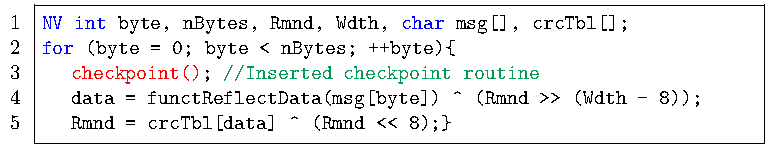
\includegraphics[width=\columnwidth]{figures/crc_example}
		\caption{Simplified C code snippet of a CRC calculation from~\cite{hicks_mibench2_2016}: per-byte message division by a polynomial; \texttt{NV} denotes non-volatile variable declaration.}\label{fig:crc_example}
	\end{subfigure}
	\begin{subfigure}[t]{\linewidth}
		\centering 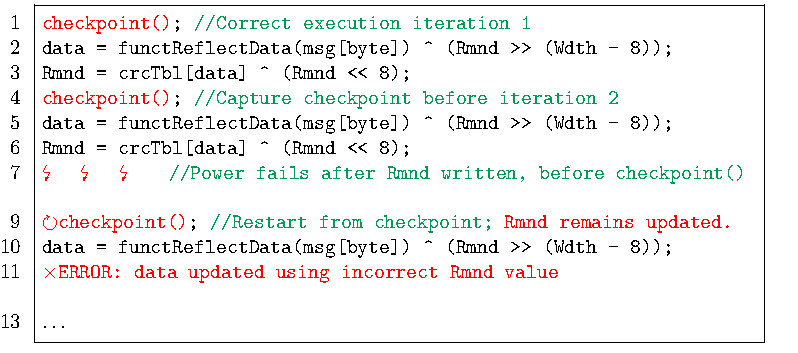
\includegraphics[width=\columnwidth]{figures/crc_example_war}
		\caption{Execution steps of the loop body in the snippet above: non-volatile checkpointing did not guarantee data consistency as data has been manipulated (line 9) with stale reminder (line 3)}\label{fig:crc_example_war}
    \end{subfigure}
	\caption{\textbf{Code example demonstrating effect of write after read on volatile memory checkpointing.}}\label{fig:code_demo_incosistency}
\end{figure}

%\begin{figure}
%	\centering
%	\subfloat[Simplified C code snippet of a CRC calculation from~\cite{hicks_mibench2_2016}: per-byte message division by a polynomial; \texttt{NV} denotes non-volatile variable declaration]{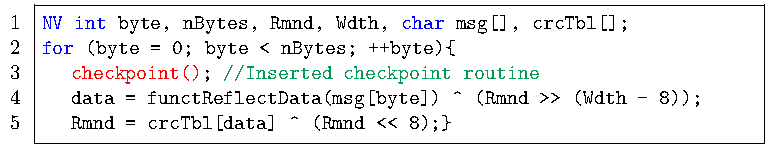
\includegraphics[width=\columnwidth]{figures/crc_example}\label{fig:crc_example}}\\
%	\subfloat[Consecutive execution steps of the loop body in the snippet above: non-volatile checkpointing did not guarantee data consistency as data has been manipulated (line 9) with stale reminder (line 3)]{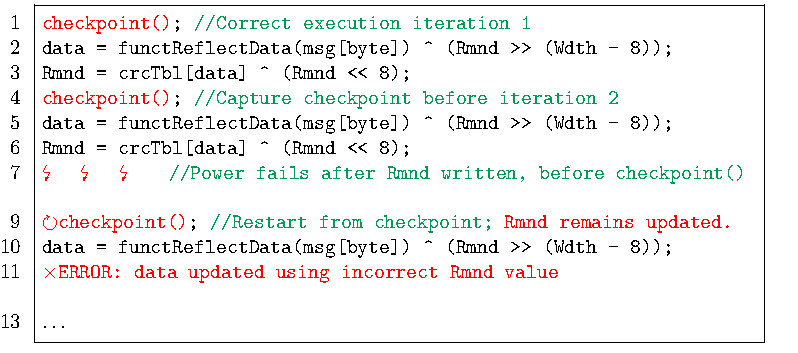
\includegraphics[width=\columnwidth]{figures/crc_example_war}\label{fig:crc_example_war}}
%	\caption{Code example demonstrating effect of write after read on volatile memory checkpointing.}
%	\label{fig:code_demo_incosistency}
%\end{figure}

Checkpoints of volatile state preserve intermittent progress, but do not ensure data consistency~\cite{dino,chain,ratchet}. Data may become inconsistent if an attempt to execute some computation {\em writes} to a non-volatile variable, then power fails, then a second attempt to re-execute the same computation incorrectly {\em reads} the value written in the first attempt, rather than the variable's original value. The situation occurs when code includes a WAR dependence between operations that manipulate non-volatile variables~\cite{ratchet,dino,alpaca}.

Figure~\ref{fig:code_demo_incosistency} illustrates how state can become inconsistent in an intermittent execution using the cyclic redundancy check (CRC) code from MIBench2~\cite{hicks_mibench2_2016}. The code computes the CRC for an $\texttt{nBytes}$ byte message $\texttt{msg}$ with remainder $\texttt{Rmnd}$.

Despite checkpointing at line 3 in Fig.~\ref{fig:crc_example}, the code may compute  $\texttt{data}$ incorrectly because of the read of $\texttt{Rmnd}$ on line 4 and the write of $\texttt{Rmnd}$ on line 5. Figure~\ref{fig:crc_example_war} shows an intermittent execution. The second iteration writes $\texttt{Rmnd}$, but power fails before the checkpoint. After restarting, line 9 reads the updated value of $\texttt{Rmnd}$, producing an incorrect $\texttt{data}$ value. Checkpoint-based systems risk violating memory consistency~\cite{dino}. To maintain consistency, prior systems~\cite{dino,ratchet} {\em version} a subset of non-volatile data with the checkpoint. Task-based systems~\cite{chain,alpaca}, which we focus on, ensure consistency using programmer, compiler, and runtime support.

\subsection{Task-based Intermittent Programming}
\label{section:background_task_computing}

Task-based execution models~\cite{dino,chain,alpaca} ask the programmer to decompose their program into tasks. A task is a function with no caller containing arbitrary computation, sensing, and communication. A programmer describes task control-flow as a {\em task graph}. Task flow happens at programmer demarcated transition points that may be conditional on program values. Task-based programming abstractions guarantee that tasks execute {\em atomically}, regardless of power failures. Task-based runtime systems ensure task-atomic semantics by ensuring that repeated task executions are idempotent. The key to idempotence is ensuring that non-volatile updates made by an interrupted task are never visible to a future task execution.  

There are several run time strategies to ensuring task idempotence. One approach~\cite{alpaca}, is to identify non-volatile data involved in WAR dependences in a task (like DINO~\cite{dino} and Ratchet~\cite{ratchet} did for checkpoints), execute the task using private copies of those data, and commit the private copies on task completion. Another way is to statically create multiple versions of non-volatile data shared by tasks and ensure that no task reads and writes the same version~\cite{chain}. Regardless of the strategy, task-based systems execute statically-defined tasks atomically, completing in one or more attempt. 

\begin{table}
	\centering
	\footnotesize
	\begin{tabular}{|c|c|}
		\hline
		Model & Data Copied to/from NVRAM \\
		\hline\hline
		Mementos~\cite{mementos}                             & Reg. + Stack     \\
		DINO~\cite{dino}                                     & Reg. + WAR variables \\
		Chain~\cite{chain}                                   & PC   + Channel data\\
		Alpaca~\cite{alpaca}                                 & PC   + WAR variables \\
		Ratchet~\cite{ratchet}, Clank~\cite{hicks_isca_2017} & Reg. (requires NV main memory) \\
		\hline
	\end{tabular}
	\caption{\textbf{Memory consistency enforcement overheads of intermittent execution models;} \emph{Reg.}: the entire register file, \emph{PC}: program counter, \emph{Channel data}: variables explicitly task-shared by the programmer, \emph{WAR variables}: variables involved in WAR dependences (\emph{NV}: non-volatile).}
	\label{table:chechpoint_comparison}
\end{table}

\subsubsection{Costs of Task-based Models}

%Task-based models incur costs that motivate \sys.

\textbf{Memory Consistency Enforcement Overhead.} Intermittent execution models incur overheads to checkpoint data~\cite{dino,ratchet,quickrecall,mementos}, manage channels~\cite{chain}, or privatize and commit data~\cite{alpaca}. Table~\ref{table:chechpoint_comparison} compares overheads for recent intermittent execution models (cf. \cite[Sec. 2.4]{alpaca}.) The mechanism responsible for overhead in each model varies, but the bulk of overhead in all models is a manipulating non-volatile memory. Checkpointing moves data to and from non-volatile memory, channel accesses manipulate non-volatile data~\cite{chain}, privatization copies from and commits to non-volatile memory~\cite{alpaca}, and idempotence solutions~\cite{ratchet} use {\em only} non-volatile memory.  

\begin{figure}
\begin{subfigure}[t]{.49\columnwidth}
	\centering 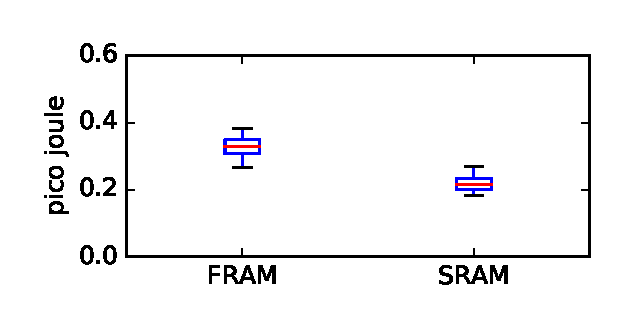
\includegraphics[width=\columnwidth]{figures/fram_write}
	\caption{Cost of \emph{write} operation}
\end{subfigure}%
\begin{subfigure}[t]{.49\columnwidth}
	\centering 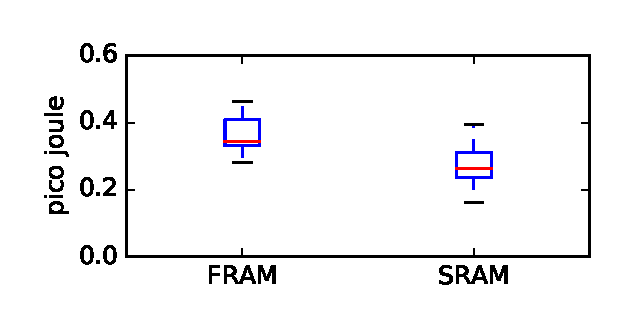
\includegraphics[width=\columnwidth]{figures/fram_read}
	\caption{Cost of \emph{read} operation}
\end{subfigure}
	\caption{\textbf{Cost of accessing volatile (SRAM)/non-volatile (FRAM) memory during write/read operation.}}\label{fig:framEnergy}
\end{figure}

%\begin{figure}
%\centering
	%\subfloat[Energy cost of \emph{write} operation]{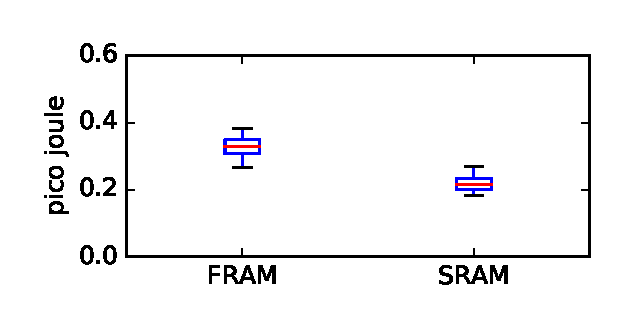
\includegraphics[width=0.49\columnwidth]{figures/fram_write.eps}}
	%\subfloat[Energy cost of \emph{read} operation]{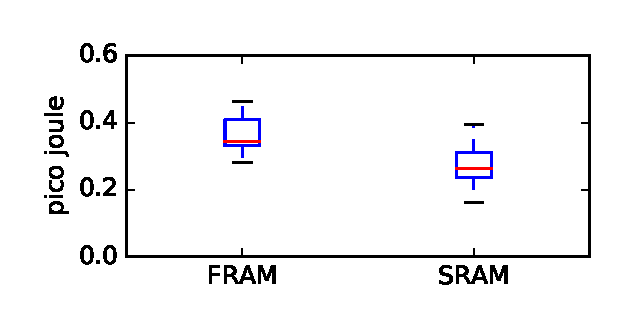
\includegraphics[width=0.49\columnwidth]{figures/fram_read.eps}}
	%\caption{Cost of accessing volatile (SRAM)/non-volatile (FRAM) memory during write (left) and read (right) operation.}
	%\label{fig:framEnergy}
%\end{figure}

To understand these non-volatile memory overheads, for the MSP430FR5969~\cite{msp430datasheet} MCU we measured the energy consumption of volatile (SRAM) and non-volatile (FRAM) memory operations. We used EDB~\cite{edb} to monitor voltage drop on a capacitor powering the device across 1600 read and write accesses to each memory type, randomizing to avoid caching. Figure~\ref{fig:framEnergy} summarizes the data, showing that a non-volatile memory access consumes around 1.5 times the energy of a volatile access in this device. In an intermittent device, energy cost corresponds to decreased run time between power failures. The cost of non-volatile memory motivates \sys, which virtualizes memory to primarily use SRAM.

%The above result reassures the intuitive observation that a decrease of checkpoint frequency (CP) decreases the energy cost associated with each state preservation method and reduces operation cost which in most simplistic terms is defined as $\mathcal{O}(\text{CP})+\mathcal{O}(\text{PL})$, where PL is the cost of program execution without checkpointing. On the other hand, this increases task/checkpoint re-execution time. The ideal solution is a runtime that \emph{adaptively} changes task size during runtime, which however exposes a second problem.

%\begin{table}
%	\centering
%	\footnotesize
%	\begin{tabular}{|c|c|}
%		\hline
%		Platform name & Storage capacitor size \\
%		\hline \hline
%		%Moo~\cite{moo} & 0.1\,F \\
%		WISPCam~\cite{naderiparizi_rfid_2015} & 6.08\,mF \\ %tested [11.24, 17.45, 21.98]\,mF
%		%NFC-WISP~\cite{zhao_rfid_2015} & 300\,$\mu$F \\
%		NeuralWISP~\cite{holleman_biocas_2008} & 100\,$\mu$F \\
%		WISP~\cite{wisp5} & 47\,$\mu$F \\
%		{\em BioImpedance} sensor~\cite{rodriguez_tbcs_2015} & 20\,$\mu$F \\
%		{\em Ingestible} sensor~\cite{nadeau_naturebio_2017} & 220\,$\mu$F\\
%		\hline
%	\end{tabular} 
%	\caption{{\em Default} energy storage sizes for example battery-less platforms. Observe a huge variation in storage capacity.}
%	%We note that values for other representative platforms~\cite{medusa_farsens_2017,talla_imwut_2017,liu_sigcomm_2013,parks_sigcomm_2014} were not reported in their respective papers.
%	\label{table:capacitor}
%\end{table}

\textbf{Fixed-size Tasks are Inflexible and Inefficient.} If a programmer writes a task that consumes {\em more} energy than the device can buffer, the task will never complete using buffered energy {\em preventing forward progress} by repeatedly re-executing. If a programmer writes tasks that consume far {\em less} energy than a device can buffer, the system may operate {\em inefficiently}. When a task and its successor both complete, the two tasks were interleaved by a task boundary that preserves progress and state (i.e., checkpoint or commit). However, absent a power failure, the work to preserve state was {\em unnecessary}, incurring overhead on the tasks' executions.

Avoiding excessively costly, non-terminating tasks and short, high-overhead tasks is a programming challenge, given fixed hardware with a fixed energy buffering capacity. Buffer sizes from prior work vary widely from 20\,$\mu $F~\cite{rodriguez_tbcs_2015} to 0.1\,F~\cite{moo}. Sizing tasks complicates {\em porting} code from one device to another. An excessively costly task on a device with a small energy buffer may be a relatively short, task on a device with a larger buffer. The key problem is that using existing systems, the programmer statically sizes tasks for a fixed energy buffer. \sys's {\em task coalescing}, described
in Section~\ref{sec:task_coalescing}, is motivated by these observations.


\section{\sys: System Overview}
\label{sec:overall_system}

\begin{figure}
	\centering
	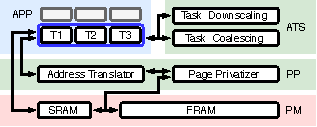
\includegraphics[width=\columnwidth]{figures/system-overview.pdf}
	\caption{\sys top-level view. ATS: adaptive task scheduler, VMM: virtual memory manager, PM: physical memory.}
	\label{fig:system_overview}
\end{figure}

\sys is a new programming and execution model for intermittent operation on energy-harvesting devices. It addresses the challenges given in Section~\ref{sec:background} making task-based intermittent applications {\em programmable}, {\em efficient} and {\em portable}, introducing a new programming model and runtime software system that supports adaptive task-based execution. Fig.~\ref{fig:system_overview} shows an overview of \sys.

\textbf{Programming and Execution Model.}  To use \sys, a programmer must (i) convert a plain C code into tasks by encapsulating the code in a top-level set of functions, (ii) sequence the control-flow between these tasks, and (iii) annotate memory accesses that manipulate task-shared data. Then, he compile the task-based code, and link to \sys's runtime, producing a \sys-enabled binary. The runtime relies on \sys's novel {\em adaptive task scheduler} to adapt its execution with the energy conditions. Facilitating efficient task adaptation requires dynamic memory protection which is \sys's \emph{virtual memory manager} through a process we call \emph{dynamic page privatization}. 

\textbf{Adaptive Task Scheduler.} \sys's adaptive task scheduler (ATS) makes \emph{energy-aware} scheduling decisions to group tasks together or split a task. By coalescing tasks \sys \emph{amortizes commit and transition costs}, and by a task splitting, after repeated failures on a single task, it \emph{avoids the task non-termination problem}. The scheduler uses its recent execution history---i.e., it is hardware independent---as a metric to estimate energy availability and eventually to decide on the coalesced task size. Section~\ref{sec:task_adaptation} describes ATS.

\textbf{Virtual Memory Manager.} \sys can coalesce tasks thanks to its virtual memory manager (VMM). VMM privatizes a group of memory pages demanded by a coalesced task and limits application accesses only to the fast volatile memory. VMM keeps all page modifications in non-volatile memory on a coalesced task transition. Section~\ref{sec:memory_virtulaization} outlines VMM.


\section{\sys: Task Coalescing}
\label{sec:task_coalescing}

\sys is able to virtually merge tasks to construct a bigger virtual task and commit the state of the virtual task instead of the individual real tasks to improve execution time at stable energy supply environment. 

\subsection{Task Merging Algorithm}

\begin{algorithm}[t]
	\caption{\sys task coalescing mechanism}
	\label{algorithm:coalescing_algorithm}
	\scriptsize
	\begin{algorithmic}[1]
		\State $\text{VT} \subset \{\sys~\text{tasks set}\}$  \Comment{Virtual task}
		\State $|\text{VT}|$ \Comment{VT size \todo{Define unit}{Amjad}}
		\State $\text{VT}_{\max}$ \Comment{Maximum VT size (With upper bound on coalescing)}
		\vspace{0.1cm}
		
		\While {True}
		\State $\text{VT} \leftarrow \text{VT}_{\text{next}}$ \Comment{\todo{Define $\text{VT}_{\text{next}}$}{Amjad}}
		\vspace{0.1cm}
		\While {execute VT} 
		\If { power failed $n$ times during task execution} \Comment{\todo{Define how it is detected}{Amjad}}				
		\State $|\text{VT}|:=|\text{VT}|-1$
		\State $\text{VT}_{\max} := |\text{VT}|$ \Comment{With upper bound on coalescing}
		\EndIf
		\EndWhile
		
		\vspace{0.1cm}
		\If {All tasks executed} \Comment{\todo{Define how it is detected and when}{Amjad}}
		\If{$|\text{VT}| < \text{VT}_{\max}$} \Comment{line added in fixed size approach}
		\State $|\text{VT}|:=|\text{VT}|+1$
		\EndIf
		\EndIf
		\EndWhile
	\end{algorithmic}
\end{algorithm}

The complete algorithm is provided in Algorithm~\ref{algorithm:coalescing_algorithm}. \todo{Fill in with missing information: scheduler description, implementation details, discussion}{Przemek/Amjad}

\subsection{Power Interrupt Immune Scheduler}

% TNT :  Total Number of Tasks
% JT 	: Total Jump
% ID	: Task ID
% D	: relative Jump (Delta)
% VCT_PT : Current Task Pointer

% if(TJ < TNT)
% 	VCT_PT <- VCT_PT + D
% else
% 	while ((dis = TJ - TNT) > TNT)
% 		dis -= ID
% 	VCT_PT <- VCT_PT + dis


\begin{algorithm}[t]
	\caption{\sys's scheduler: relative jump algorithm}
	\label{algo:relativeJump}
	\scriptsize
	%\small
	\begin{algorithmic}[1]
			\State \textsf{TNT}: Total Number of Tasks
			\State \textsf{ID}: Task ID
			\State \textsf{$\delta$}: Relative Jump
			\State $\textsf{TJ} \leftarrow (\textsf{ID} + \delta )$ \Comment{Total Jump}
			\State \textsf{\textsf{$VCT_{pt}$}}: Virtual Current Task Pointer

			\If { \textsf{TJ} > \textsf{TNT} }
				\State $\textsf{dis} = \textsf{TJ} - \textsf{TNT}$
				\While{ $ \textsf{dis} > TNT $ }
					\State $\textsf{dis} -= \textsf{TNT}$
				\EndWhile
				\State $\textsf{dis} -= \textsf{ID}$
				\State \textsf{$VCT_{pt}$} $+= \textsf{dis}$
			\Else
				\State \textsf{$VCT_{pt}$} $+= \delta $

			\EndIf
	\end{algorithmic}
\end{algorithm} %Task jumping algorithm

It utilizes a persistent circular buffer (i.e. persistent linked list) to keep the state of a program across power failures. \sys provides an API to enable a programmer to have a full control over the execution flow of the program, i.e. (un)blocking a task or re-execute the same task which is particularly important in the intermittent execution to emulate a persistent loop. \todo{Expand this section}{Amjad}

%\begin{algorithm}
%	\caption{Opportunistic virtual Task size}
%	\label{algo:fixVirtTask}
%	\scriptsize
%	%\small
%	\begin{algorithmic}[1]
%		\State $VT \subset \text{\{\sys Tasks\}} $  \Comment{$VT:$ Virtual Task}
%		\State VTS : VT size
%		\vspace{0.1cm}
%		
%		\While {$True$}
%		\State $VT \leftarrow VT_{next}$
%		\vspace{0.1cm}
%		\While {execute $VT$} 
%		\If { $\text{power failed twice}$ }				
%		\State $VTS--$  
%		\EndIf
%		\EndWhile
%		
%		\vspace{0.1cm}
%		\If {$ \text{All tasks executed}$}
%		\State $VTS++$
%		\EndIf
%		\EndWhile
%	\end{algorithmic}
%\end{algorithm}

\section{\sys: Memory Virtualization}
\label{sec:memory_virtulaization}

% \textcolor{red}{[additional motivation for coala memory virtualization] we should emphasize that Coala programming model removes the burden of identifying the write-after-read dependencies from the programmer  as compared to Chain. And it does not require a specific compiler that cannot consider a runtime dependent behavior like Interrupts service handling to guarantee memory protection, as in Alpaca.}

\sys's {\em virtual memory manager} exposes non-volatile memory for
\emph{protected} variables to the application as a virtual address space
partitioned into pages.
%
A program's tasks read and write these protected variables, using them like any
other data in the program.
%
The virtual memory manager automatically finds a variable in its page and
allows a task to directly manipulate its value.
%
When a task completes, the virtual memory manager ensures that updated pages
are committed to main memory and visible to subesequently executed tasks.
%
If a power failure interrupts a task, the virtual memory manager ensures that
the task sees consistent memory state when it restarts its execution.
%
The virtual memory manager ensures consistency even if a task or a sequence of tasks include WAR dependences that could compromise consistency~\cite{ratchet,dino}.
%
%
%
%,. Virtualization simplifies
%coalescing, because the system gets the freedom to move application's data
%between volatile and non-volatile memory transparently.
%

\sys's virtual memory manager \sys abstracts non-volatile storage (e.g.,
variables in FRAM) from tasks, which simply manipulate protected variables.
%
Protected variables remain consistent and are durable across power failures.
%
While ensuring variables remain durable, \sys avoids accessing non-volatile
memory when possible, by copying pages of data into a {\em working memory} in the device's SRAM, which
has a lower latency and energy cost to access than the device's FRAM (as we
showed in Section~\ref{sec:background}).
%
%
On a commit, \sys atomically copies all updated (i.e., ``dirty'') pages from their
space in the working memory back into their location in the non-volatile
memory.
%
SRAM has a limited size and there is an extended working memory containing {\em
shadow pages} in the larger FRAM.  A shadow page stores the data from an
updated pages that need to be committed back to non-volatile memory, but that
exceeded the size of the volatile working memory.
%
%manages memory such that application tasks operate primarily from
%efficient volatile SRAM rather than non-volatile FRAM, which is more costly to access than SRAM,
%as we showed in Figure~\ref{fig:framEnergy}.
\sys moves pages of data efficiently using hardware accelerated Direct Memory
Access (DMA) support, which copies a block of memory from one place to another
as a single operation.


\begin{figure}
	\centering
	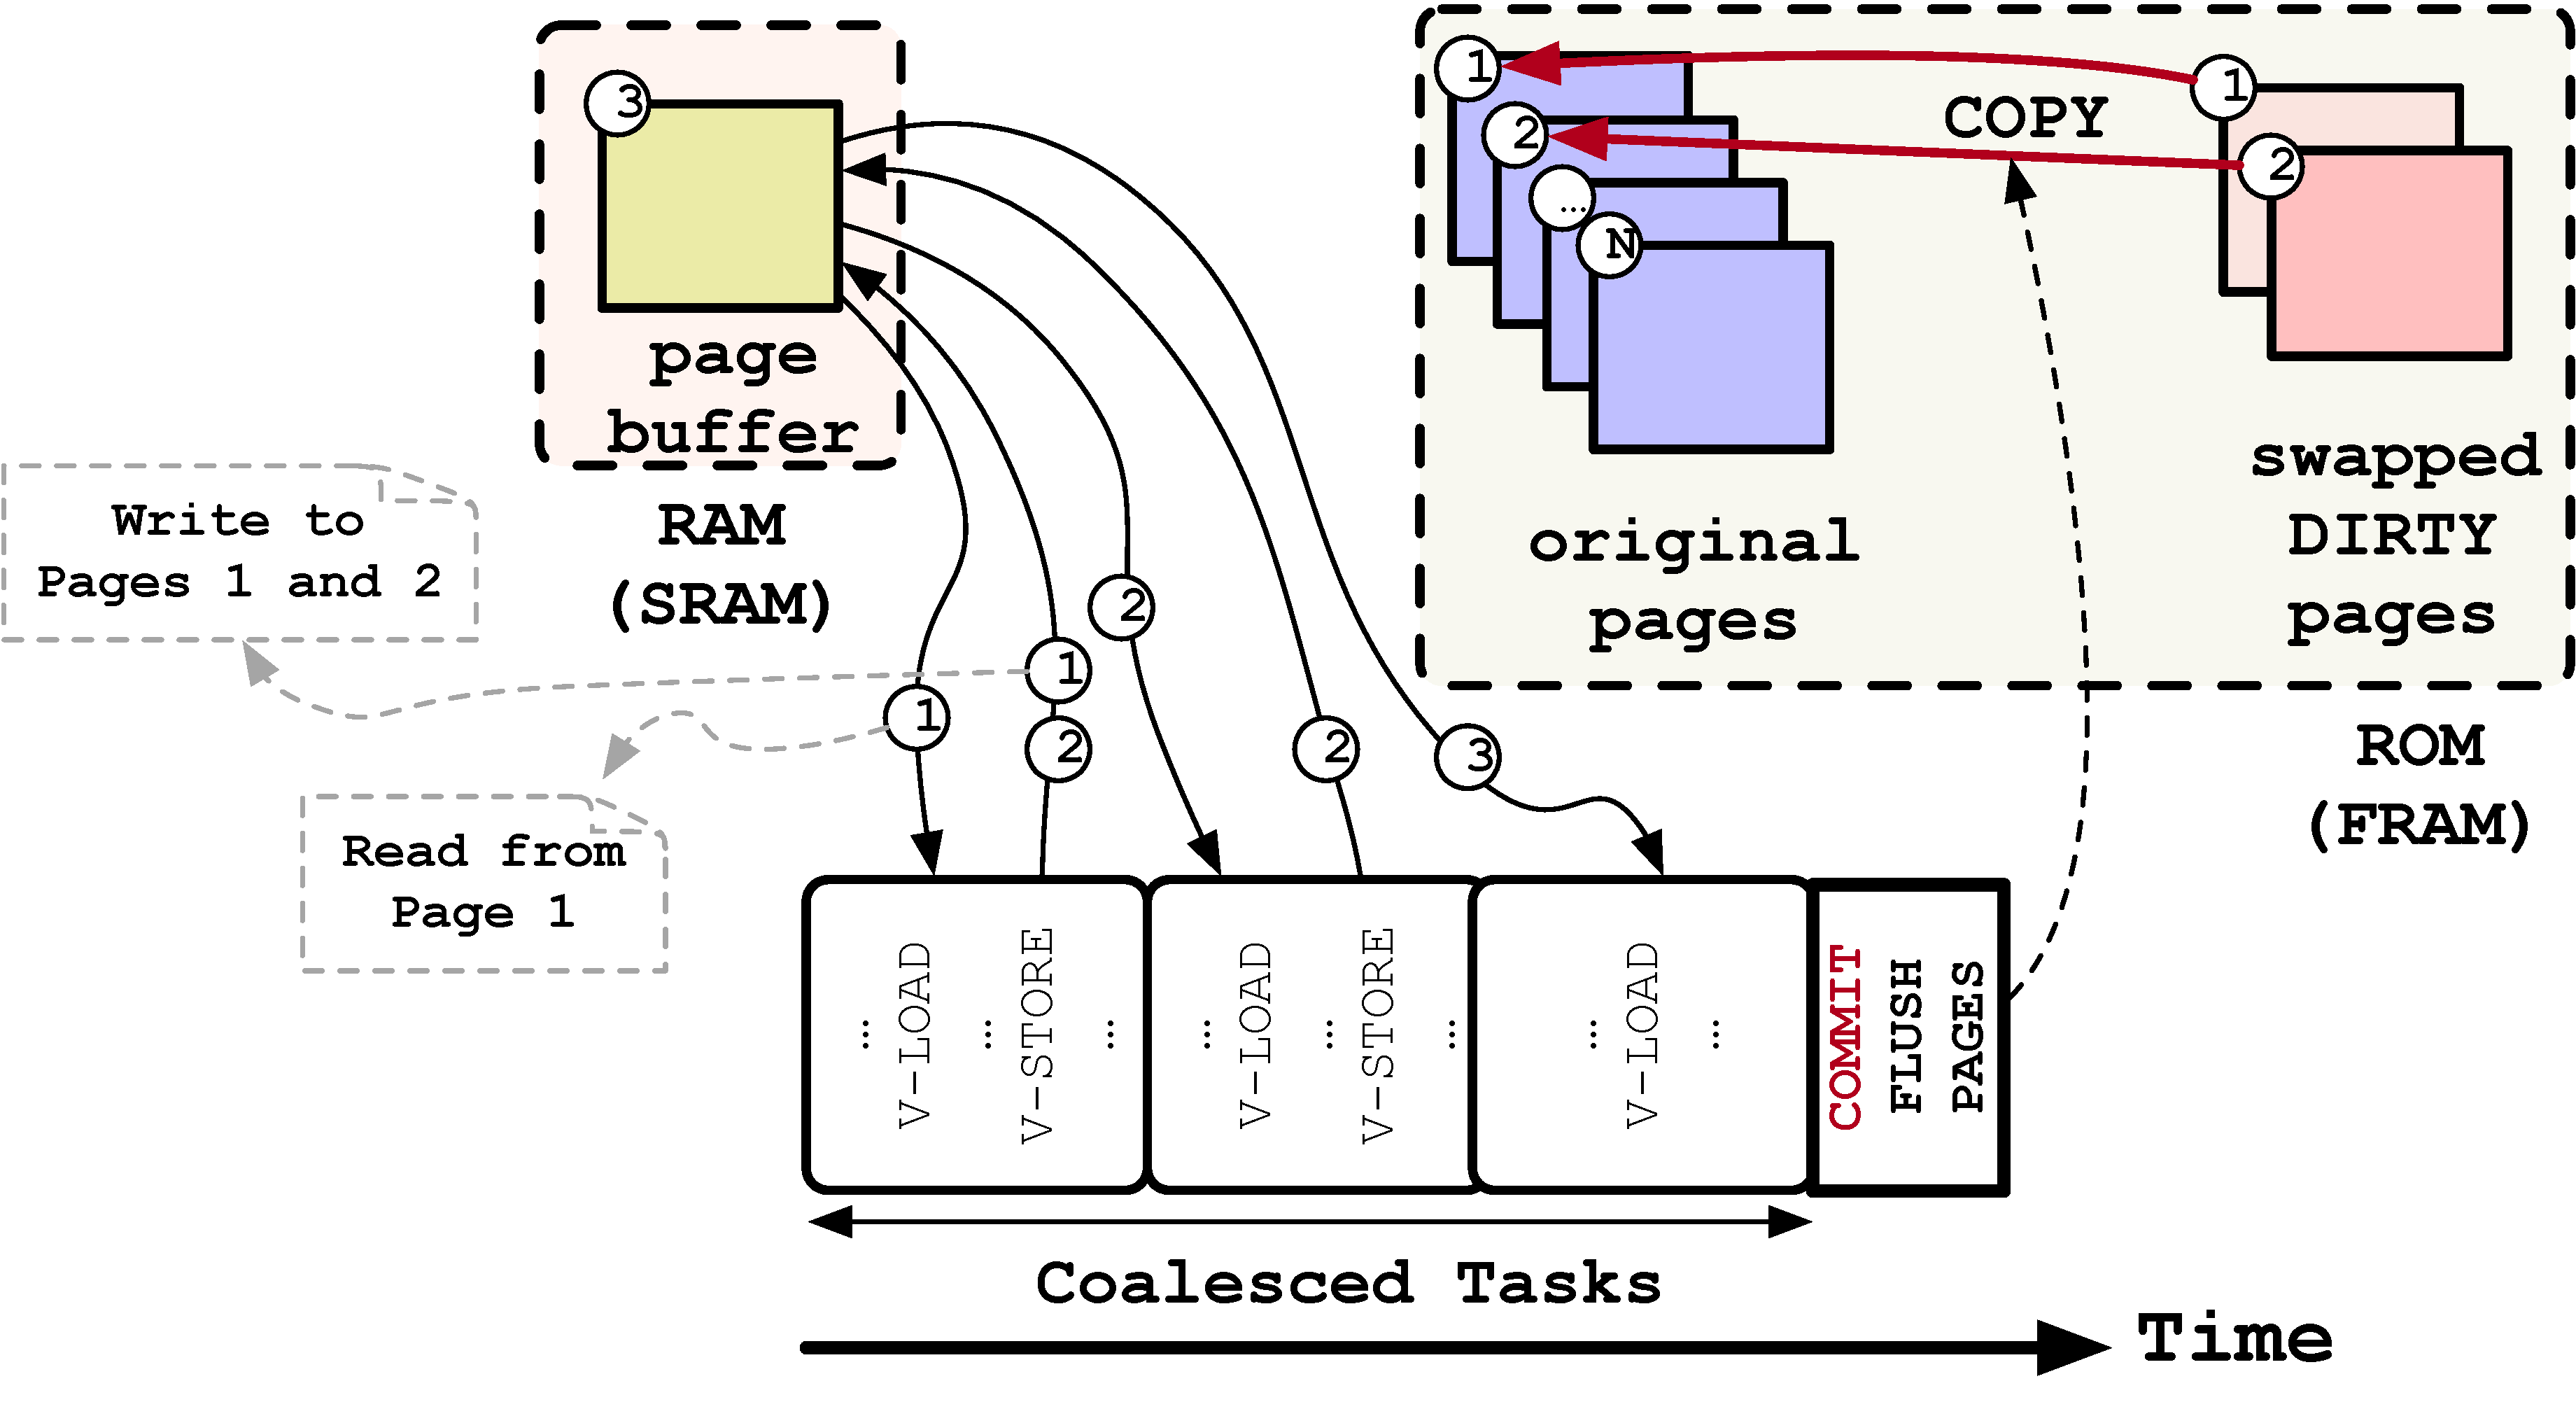
\includegraphics[width=\columnwidth]{figures/paging.pdf}
	\caption{Illustration of task-virtual memory interaction in \sys. Tasks only interact with the working buffer in SRAM (indicated as page buffer). The shadow buffer is used to hold the dirty bages. The indirection table is used to speed-up two-phase commit operation: it eliminates the copy operation in the second phase.}
	\label{figure:coala_page_tags}
\end{figure}

\textbf{System Overview.} Figure~\ref{figure:coala_page_tags} provides an
overall view of \sys's virtual memory management system.  A page has a home
location in non-volatile memory which we refer to as the page's
\texttt{\underline{store}} (underlined locations are non-volatile).  When a
task accesses a page, the memory manager swaps the page from its home location
into the fully\hyp{}associative \texttt{working} buffer that is stored in
volatile memory.  The \texttt{working} buffer is allocated to take up the
volatile memory that remains after space for stack is allocated.
%
\sys uses a two-phase commit to write dirty pages from the \texttt{working}
buffer back to their home location in \texttt{\underline{store}} atomically,
ensuring data consistency even in the presence of a power failure during commit.
%
The memory manager is forced to swap out a dirty page from the \texttt{working} buffer
when a task accesses a page that is not in the working buffer, and there is no
free page in the working buffer (i.e., a page fault). On a page fault, \sys
moves the page to a direct\hyp{}mapped non-volatile \texttt{\underline{shadow}}
page buffer. Later, to commit the page, \sys writes it from its
\texttt{\underline{shadow}} location back to its home location in
\texttt{\underline{store}}.
%
%BML: this point is true, but without caches, it is not a performance factor, so I removed it.
%Unlike prior work~\cite{chain,alpaca} that moves scattered variables one at a
%time between volatile and non-volatile memory, \sys's page-based design moves
%contiguous blocks of data.
%
%BML: this seems gratuitous because DMA is very common and we've already introduced it.
%\sys takes full advantage of hardware\hyp{}accelerated block copies using
%Direct Memory Access (DMA) hardware in common microcontrollers --- e.g.
%5$\times$ fewer cycles on MSP430FRxxxx.

\subsection{Address Translation and Variable Access}

A \sys task must access protected non-volatile variables through \sys's
restricted memory interface, which Section~\ref{sec:coala_api} describes in
detail.  The interface includes \texttt{RP(var)}, to read the value of variable
{\tt var}, and \texttt{WP(var)} to assign a value to variable {\tt var}. The
implementation of {\tt RP} is shown in Algorithm~\ref{algo:rwar}, and {\tt
WP}'s implementation is similar except that {\tt WP} marks the accessed page as
dirty.
%
{\tt RP} and {\tt WP} operations translate a variable's physical address in
non-volatile memory into a \emph{virtual address} in the page buffer in
volatile memory. In \sys, a virtual address is composed of a \emph{page tag}
that identifies the page and a \emph{page offset} that identifies a byte.

%How an $a$-bit memory address decomposes into a tag and an offset depends on the number (and size) of each page of protected memory. To address {\tt p} pages of size {\tt s}, a tag comprises $log(p)$ bits, the offset comprises $log(s)$ bits and $log(p) + log(s) = a$. For example, in a 16-bit address space (i.e., 16\,kB of protected memory) with 512 pages of 128 bytes each, a page's tag is the high-order nine bits of the address and a byte's page offset is the remaining 7 bits.

%\begin{algorithm}[t]
\begin{figure} %{t}{0.4\textwidth}
\fbox{\parbox{\linewidth}{
	\captionof{algorithm}{\texttt{RP}(variable $v$)}
	\label{algo:rwar}
	\scriptsize
	%\small
	\begin{algorithmic}[1]
		\State $t \leftarrow \Call{GetTag}{v}$
        \State $i \gets \{ j\ |\ \Call{GetTag}{\texttt{working}[j]} = t \}$ \Comment{Search page}
		\If { $i = \emptyset$ } \Comment{Var in a resident page?}
		\State	$i \gets \Call{PageFault}{t}$ \Comment{Swap page in}
		\EndIf
		\State $o \leftarrow \Call{GetOffset}{v}$
		\State \Return \texttt{working}[$i$][$o$]  \Comment{Return from page}
%	\end{algorithmic}
%\end{algorithm}
	\end{algorithmic}}}
\end{figure}

After address translation, \sys attempts to access the protected variable's
location in the volatile paging buffer. \sys keeps track of the page tags for
the pages currently resident in the paging buffer. When a task accesses a
variable, it compares the variable's page tag to tags of the pages in {\tt
working} (Line 2).
%
%If the accessed variable's page is resident in the page buffer,
%then the tag of one of the pages in this buffer is equal to the accessed
%variable's page tag.
%
If the accessed variable's page tag is not found in the page buffer, the
operation incurs a {\em page fault} (Line 4). At a page fault, \sys must swap
out one of the pages that is resident in the page buffer (to the non-volatile
\texttt{\underline{shadow}}) if \texttt{working} is full, and swap in the
variable's page.
%
The byte is accessed in the page buffer at the index of the resident page and
the variable's page offset (Lines 5--6).

%Algorithm~\ref{algo:rwar} shows pseudo-code of \texttt{RVAR} and we omit a listing for {\tt WVAR} as it is very similar except it writes the memory location and returns nothing. If the page tag of the variable \texttt{var} is not found in \texttt{working} (e.g. Lines 2--3), there is a page fault that requires a new page to be swapped in to the page buffer.

\subsection{Page Faults and Page Swapping}

If the \texttt{working} buffer is full, a page fault on a memory access
requires \sys to swap out one of the pages in the volatile buffer (a
\emph{victim page}) preserving updates made to that page, and to copy the
accessed page of protected data into the working buffer.
Algorithm~\ref{algo:pagefault} shows how \sys handles a page fault. A victim
page in the \texttt{working} buffer is selected for eviction according to
a \emph{first-in-first-out} (FIFO) replacement policy (Lines 2 and 12).
%
While we opted for the simplicity of FIFO, any other replacement policy, such
as Least Recently Used (LRU) could work in its place.

% \begin{algorithm}
% \begin{wrapfigure}{t}{0.5\textwidth}
% \fbox{\parbox{}{
% 	\captionof{algorithm}{\texttt{PageFault}(tag $t$)}
% 	\label{algo:pagefault}
% 	\scriptsize
\begin{algorithm}
	\caption{\texttt{PageFault}(tag $t$)}
	\label{algo:pagefault}
	\scriptsize
	%\small
	\begin{algorithmic}[1]
        \State \LeftComment{$i_\text{victim}$: index to free slot or page to be evicted, initially 0}
        \State \LeftComment{\texttt{\underline{shadowCount}}: non-volatile, 0 on boot unless in phase 2 commit}
        \State $t_\text{victim} \gets \Call{Tag}{\texttt{working}[i_\text{victim}]}$
		\If {\Call{isDirty}{working[$i_\text{victim}$]} }	\Comment{Evicting a dirty page?}
		\State $\texttt{\underline{shadow}}[t_\text{victim}] \xleftarrow{\text{DMA}} \texttt{working}[i_\text{victim}]$
            \Comment{Swap out the page}
        \If {$t_\text{victim} \not\in \texttt{\underline{shadowList}}$} \Comment{Keep track for quick traversal}
            \State $\texttt{\underline{shadowList}}[\texttt{shadowCount++}] \gets t_\text{victim}$
        \EndIf
		\EndIf
		\If {\Call{exists}{\underline{shadow}[$t$]}} \Comment{Page swapped out earlier?}
		\State $\texttt{working}[i_\text{victim}] \xleftarrow{\text{DMA}} \texttt{\underline{shadow}}[t]$
            \Comment{Get from commit buffer}
		\Else
		\State $\texttt{working}[i_\text{victim}] \xleftarrow{\text{DMA}} \texttt{\underline{store}}[t]$
            \Comment{Get from backing store}
		\EndIf
        \State $i_\text{victim} \gets (i_\text{victim} + 1) \mod |\texttt{pageBufLength}|$ \Comment{FIFO evict}
	\end{algorithmic}
\end{algorithm}

% 	\end{algorithmic}
% \end{algorithm}
	% \end{algorithmic}}}
% \end{wrapfigure}

If a task modified any byte in the victim page (i.e., using \texttt{WP}), then
the page is dirty.  If the page being swapped out is not dirty and the page
being accessed had not been dirtied and swapped out to the \texttt{shadow}
buffer since the last reboot, then handling a page fault requires copying the
accessed page from its home in the  \texttt{\underline{store}} into the
\texttt{working} buffer (Line 11).  Otherwise, the page fault handler must take
the following extra steps.
%
Before swapping in the accessed page, \sys must first preserve the updated
values in the dirty page so that they can be committed back to their locations
in memory when the task commits (but not earlier).  To preserve the dirty
values, \sys copies the victim page to the non-volatile
\texttt{\underline{shadow}} buffer (Line 5) and records the page's tag in a
non-volatile commit list (Lines 6-7). \sys uses the commit list to iterate over shadow pages
at commit time, to copy the contents of shadow pages back to the main memory {\tt store}.
%
%Dirty pages remain in {\tt \underline{shadow}} buffer until the
%dynamic task completes, at which point \sys commits the modified
%pages from {\tt \underline{shadow}} back to \texttt{\underline{store}}.
%
If the accessed page was previously modified and swapped out since the last
power failure (Line 8), the most recent version of the page is in {\tt
\underline{shadow}}, not \texttt{\underline{store}} (Line 9).



%As
%Algorithm~\ref{algo:pagefault} shows in Line 4, \sys checks if the requested
%page was previously modified by the executing task. To track whether a page is
%modified, \sys stores a dirty bit with the page and sets it when the page is
%written to. If an accessed page's dirty bit is set, the page must be swapped in
%from \texttt{\underline{shadow}} rather than its original memory location (Line 5),
%furnishing the task with the page's modified values. If the accessed page is
%not dirty, \sys swaps it in from its original location in memory (Line 7).

%
%\sys
%uses DMA block copies for all page swapping operations, leveraging the
%efficiency of hardware support.

\subsection{Atomic Two-Phase Commit of Dirty Pages}

When the last task in a sequence of coalesced tasks completes, \sys must commit
\emph{all} dirty pages in the \texttt{working} buffer and in the
\texttt{\underline{shadow}} buffer, copying them back to their original
locations in the main memory \texttt{\underline{store}}. If a task were allowed
to (re-)execute after only some pages have been committed to
\texttt{\underline{store}}, the task might see protected variables in an
inconsistent state; \sys's two-phase commit prevents this inconsistency.

To make the commit atomic, \sys commits the pages in two phases, implemented by
Algorithm~\ref{algo:commit}.
%
The first phase copies dirty pages from the \texttt{working} buffer to the
non-volatile \texttt{\underline{shadow}} buffer (Line 4). The second phase
commits pages from \texttt{\underline{shadow}} to \texttt{\underline{store}}
(Line 12).  If power fails during the first phase, the whole commit is aborted,
and the execution restarts from the most recently committed point (i.e., from
the first task in a coalesced sequence of tasks). If power fails in the second
phase, the commit process safely resumes on reboot.  The second phase of commit
depends on some run-time metadata. The \texttt{\underline{committing}} bit
indicates that a commit is in progress and is set before the first page is
committed (Line 9) and cleared after the last page is committed (Line 16).  The
\texttt{\underline{shadowCount}} records the number of dirty shadow pages to
commit and \sys clears the counter when commit completes (Line 14).  The
\texttt{\underline{commitIndex}} indexes the next page to be committed (Line
11) and \sys clears the index at the end of the phase (Line 15).
%
\sys's commit is efficient because it maintains an index dirty pages instead of
iterating through all potentially dirty pages to check a dirty bit during
commit.
%
\sys's implementation is also efficient because the memory manager does not
copy from \texttt{\underline{shadow}} to \texttt{\underline{store}}, instead
swapping pointers in an indirection table that maintains the pages as a double
buffer.  Section~\ref{sec:implementation} describes double buffering in more
detail.

%\subsection{Paging Example}
%
%Figure~\ref{fig:volatile-buffer} illustrates the execution of a simple task using \sys's paging mechanism. The task manipulates the protected variables {\tt x}, {\tt y}, and {\tt z}. The variables {\tt y} and {\tt z} are in the same page and they are currently in the volatile page buffer---on accessing {\tt y} and {\tt z}, the task needs only to access \texttt{pageBuf}. Since variable \texttt{x} is kept in a different page in \texttt{pagesOrg}, accessing it creates a page fault. At this point, \sys swaps the active page in \texttt{working} by committing it into the non-volatile {\tt \underline{shadow}} region and copying the corresponding page from \texttt{pagesOrg} to \texttt{pageBuf}. When the task completes, \sys sets the commit bit, copies the dirty page from \texttt{pagesTmp} to its original location in \texttt{pagesOrg} and unsets the commit bit.

%\begin{figure}[t]
%	\centering
%	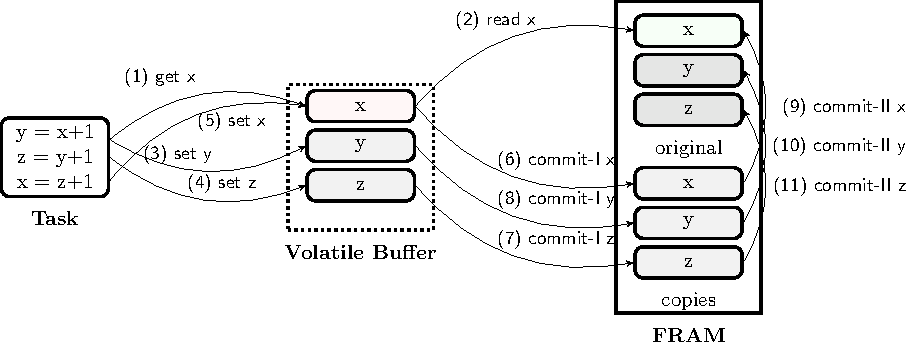
\includegraphics[width=0.75\columnwidth]{figures/sram-buffer}
%	\caption{The interaction between the task, volatile buffer and the non-volatile memory (FRAM). Initially, the persistent variable \texttt{x} is not in the volatile buffer but \texttt{y} and \texttt{z} are.}
%	\label{fig:volatile-buffer}
%\end{figure}

%\subsection{Memory Consistency}

\textbf{Memory Consistency.} \sys's paging mechanism ensures that a task only
ever executes using consistent protected data. During task execution,
modifications to protected data do not affect their original memory locations,
because a task reads and writes the volatile \texttt{working} buffer only, and
modified pages are kept in \texttt{\underline{shadow}} until commit.  A power
failure erases the contents of the page buffer, preventing a re-executing task
from observing updates in the page buffer from a previous execution attempt.
Clearing \texttt{\underline{shadowCount}} as part of the second phase commit
(Line 14), ensures that all accesses to protected variables in subsequent tasks
correctly access their original memory locations in \texttt{\underline{store}}.
\sys assumes that the write to a non-volatile word in memory is atomic.
%
%The non-volatile commit bit persists
%across power failures and \sys repeatedly attempts to commit until it succeeds,
%despite arbitrary power failures.

%\begin{algorithm}[t]
% \begin{wrapfigure}{t}{0.5\textwidth}
% \fbox{\parbox{\linewidth}{
% 	\captionof{algorithm}{Two-phase commit}
% 	%\caption{Two-phase commit}
% 	\label{algo:commit}
% 	\scriptsize

\begin{algorithm}[t]
	\caption{Two-phase commit}
	\label{algo:commit}
	\scriptsize
	%\small
	\begin{algorithmic}[1]
        \Procedure{CommitPhase1}{} \Comment{On last coalesced task}
            \For {$i \in 0..|\texttt{working}|-1$}
                \State $t \gets \Call{Tag}{\texttt{working}[i]}$
                \State $\texttt{\underline{shadow}}[\Call{Tag}{\texttt{working}[i]}] \xleftarrow{\text{DMA}} \texttt{working}[i]$
                \State $\texttt{\underline{shadowList}}[\texttt{\underline{shadowCount}}] \gets t$
                \State $\texttt{\underline{shadowCount}} \gets \texttt{\underline{shadowCount}} + 1$
            \EndFor
            \State \Call{CommitPhase2}{}
        \EndProcedure
        \Procedure{CommitPhase2}{} \Comment{\texttt{\underline{commitIndex}} 0 on first boot}
            \State $\texttt{\underline{committing}} \gets \textbf{true}$
            \While{\texttt{\underline{commitIndex}} < \texttt{\underline{shadowCount}}}
                \State $t \gets \texttt{\underline{shadowList}}[\texttt{\underline{commitIndex}}]$
                \State \Call{commitToStore}{\texttt{\underline{shadow}}[t]}
                \State $\texttt{\underline{commitIndex}} \gets \texttt{\underline{commitIndex}} + 1$
            \EndWhile
            \State $\texttt{\underline{shadowCount}} \gets 0$
            \State $\texttt{\underline{commitIndex}} \gets 0$
            \State $\texttt{\underline{committing}} \gets \textbf{false}$
        \EndProcedure
        \Procedure{OnBoot}{} \Comment{Invoked on every boot}
            \If { \texttt{\underline{committing}} } \Call{CommitPhase2}{}
            \EndIf
            \State $\texttt{\underline{shadowCount}} \gets 0$, $i_\text{victim} \gets 0$
        \EndProcedure
	\end{algorithmic}
\end{algorithm}
% 	\end{algorithmic}}}
% \end{wrapfigure}



\subsection{Dynamic Paging of \sys}

\sys asks the programmer to use its {\tt RP} and {\tt WP} paging API methods on
every access to a protected variable (cf. Section~\ref{sec:coala_api}).  These
API invocations present a risk of high overhead because there is a dynamic
check on every read and write. An alternative approach~\cite{alpaca} relied on a compiler to analyze memory operations and try to insert memory protection code mostly at the beginning of a task, leaving most
memory accesses uninstrumented.

Despite the risk of per-access overhead, \sys's dynamic memory protection
scheme brings several benefits over a static approach.  First, the limitations
of static analysis preclude some uses of pointers due to potential pointer
aliasing. For example, in the presence of arbitrary pointer operation, a
function call using a function pointer, or an interrupt within a task, the
system cannot statically analyze the memory behavior.   Second, a static approach
cannot handle task coalescing, because a protected variable's lifetime (i.e.,
from first use to commit) is unknown at compile time. \sys's dynamic,
per-access instrumentation supports arbitrary use of pointers and enables task
coalescing.
%
%Moreover, if the programmer wants to optimize for high performance, it is possible for the
%programmer to place {\tt RP} and {\tt WP} only minimally by carefully examining the code.
%We argue that the


%\TODO{Put paragraph about Alpaca's static privatization algo vs. Coala's dynamic privatization algo}
%\TODO{pass by ref might not work the right way}
%\begin{verbatim}
%
%GLOBAL_(x)
%
%foo(*y){
%  *y++;
%}
%
%TASK( ){
%  ... ;
%  foo( &GV(x) ) ;
%}
%
%\end{verbatim}
%\subsection{Managing Paging Overhead}
%
%The efficiency of \sys's paging scheme relies on the fact that data in pages are contiguous, which makes them amenable to being manipulated by hardware assisted DMA bulk copy operations. To justify this design choice we experimentally evaluated the efficiency of using DMA block copies, compared to explicit, software copy loops. We copied blocks of data of different size between memory regions on a WISP~\cite{wisp} using a hand-written loop and using DMA (refer to Section~\ref{sec:results_hardware} for hardware setup details). Figure~\ref{fig:dmaTimeEnergy} shows that for moving large blocks of data like a page, hardware DMA is considerably better than software in both run time and energy efficiency. \sys's design moves data in pages, not individual words, leveraging the increased efficiency of DMA data movement.
%
%\begin{figure}[t]
%	\centering
%	\subfloat[Time needed to transfer a block of data]{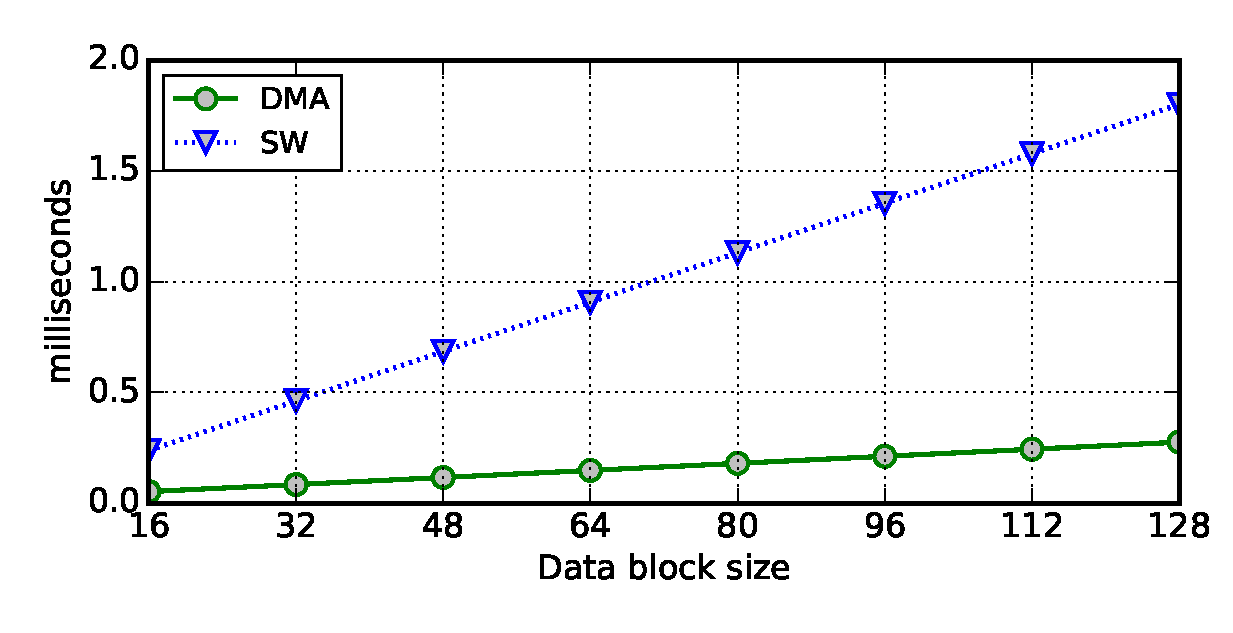
\includegraphics[width=0.49\columnwidth]{figures/dmaSize_time.eps} }
%	\subfloat[Energy needed to transfer a block of data]{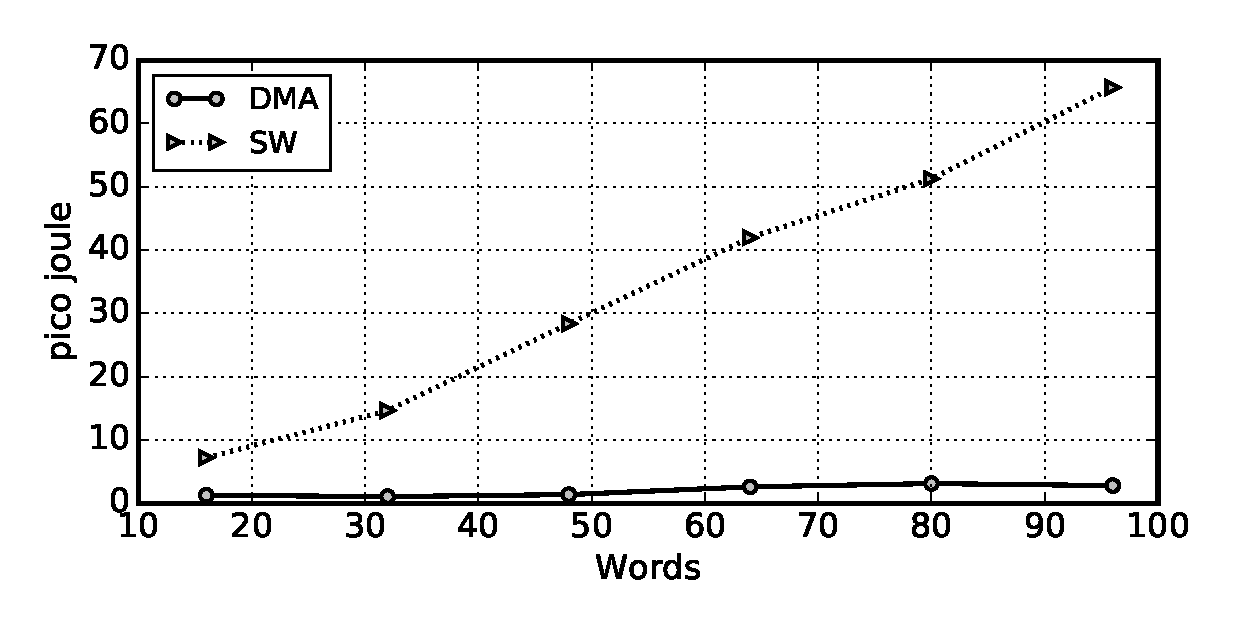
\includegraphics[width=0.49\columnwidth]{figures/energyConsumptionDMA_SW.eps}}
%	\caption{Time and energy consumption of moving a block of data from SRAM to FRAM: CPU intervention versus Direct Memory Access (DMA).\todo{Explain HW/SW setup; make fonts larger, unify legends and axes}{Amjad}}
%	\label{fig:dmaTimeEnergy}
%\end{figure}



\section{\sys: Automatic Task Generation}
\label{sec:compiler}

We studied \sys's effectiveness for systems with automatically generated task
boundaries by developing a simple compiler prototype that transforms an
arbitrary C into a program with tasks. The compiler is representative of,
although \emph{not a direct implementation} of, a system that assists in writing
task-based programs by automatically inserting tasks (e.g., inspired by
Ratchet~\cite{ratchet}). 

\textbf{Automatic Task Generation Flow.} Transforming C code to use tasks requires identifying program points to use as task boundaries, defining a set of task functions that begin and end at those boundaries, ensuring that all existing control-flow paths are either contained within a task or are made explicit with inter-task control-flow, and identifying and instrumenting accesses to task-shared variables that need to be protected by \sys at runtime. Our simple prototype, implemented using LLVM, analyzes the control-flow graph (CFG) and uses a rule-based heuristic to determine where to place a task boundary. After identifying task boundaries placement, the \sys compiler transforms the imperative code into tasks, instrumenting protected memory accesses. 

\subsection{Task Boundary Identification Analysis}
\label{sec:compiler_analysis_pass}

\sys analyzes a program to determine where to put task boundaries. A task is single-entry, multiple-exit part of the CFG that \sys compiler excises into a new function. There are several factors determining efficient task execution. A task decomposition should minimize the number of variables that are accessed by multiple tasks and, consequently, must be protected by \sys's paging mechanism. Different tasks should be approximately the same size to make reasoning about coalescing simple by eliminating the need to consider variable run time costs. To minimize task boundary overheads (e.g., commit), a task decomposition should maximize task size, which minimizes the frequency of task transitions.

%\begin{enumerate}[label={\bf C\arabic*:}]
%\item{No task should ever use up more energy than what the capacitor of the system can provide;} \TODO{We do not (cannot, actually) guarantee this, so I think we can, at best, say that this is an optimization constraint.  What do you think?}
%\item{A task should be single-entry.}\todo{Define single entry}{Kiwan} 
%\end{enumerate}
%
%For a task-decomposition to be efficient, the compiler should optimize the following points:
%
%\begin{enumerate}[label={\bf O\arabic*:}]
%\item{Tasks should be roughly the same size for efficient coalescing;}
%\item{The number of protected variables should be minimized;}
%\item{Task boundary should be visited as least as possible due to overhead on boundaries.}\todo{Define overhead on boundaries}{Kiwan}
%\end{enumerate} 

%\sys meets these correctness and efficiency requirements with a four-part analysis composed of (i) \emph{graph construction}, (ii) \emph{loop analysis}, (iii) \emph{task preparation}, and (iv) \emph{single entry assurance}.

\begin{figure}
	\centering
	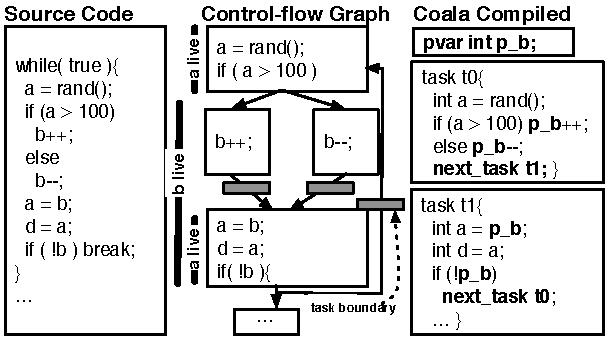
\includegraphics[width=\columnwidth]{figures/compiler.pdf}
	\caption{\sys compiles code to use tasks.}
	\label{fig:compiler_overview}
\end{figure}

The task boundary identification analysis processes a standard C program (as
shown in Figure~\ref{fig:compiler_overview}) and produces a CFG with some vertices marked as {\em task boundaries}. In our simple reference prototype, we implemented inter-procedural analysis by inlining all functions called. We opted not to support recursion, which is uncommon in embedded code. We leave to future work better approaches to inter-procedural analysis and task transformation.

%\sys uses a cost-based task boundary placement analysis that considers per-block energy consumption estimates, inter-task variable liveness, and the cost of partitioning loops.

\subsubsection{Task Cost Analysis}

\sys's task cost analysis considers estimated run time, the liveness of
variables and the cost of splitting loops across tasks. The result of the task
cost analysis determines where to place boundaries in the CFG.
 
\textbf{Estimated Run Time.} \sys assigns each basic block in the CFG a
{\em cost}, i.e. an estimate of the run time of the block. Precisely
modelling the run time and energy cost of arbitrary C code is difficult and
beyond the scope of our simple compiler prototype. Instead, our prototype counts
LLVM intermediate representation (IR) instructions and assigns a higher cost to
a block with more operations, assuming that the block runs for a longer period
of time and consumes more energy. To make the cost estimate useful, our compiler prototype estimates the maximum cost that the device's energy buffering capacitor supports. \sys does this by measuring the number of arithmetic operations that can execute without a power interruption, starting from a full capacitor. This maximum number of operations is a limit on the cost of a task---any longer task risks not executing to completion.

\textbf{Live Variable Cost.} Each CFG edge associates with a set of
variables that {\em may} be {\em alive} across the edge, i.e. variables
assigned before the edge and may be read after the edge. Variables that live
across an edge must be protected by \sys's memory virtualization when
\sys places a task boundary on the edge. \sys heuristically minimizes variable
virtualization overhead by placing boundaries to minimize the number of
live variables that span task boundaries.

\textbf{Loop Cost.} Loops are a challenge for \sys because the analysis
must account for the cost of multiple iterations of the loop body. \sys assumes
that most loops are annotated with a static loop bound. For loops that do not
have a static bound, \sys conservatively assumes the loop will be too large to
fit within a single task. Assuming loop bounds is a reasonable simplification:
while not always the case, long loops in embedded code are often statically
bounded, especially when code aims to meet strict resource requirements. 

%removed statement "which is common in embedded code"

The analysis tries to minimize the dynamic overhead of traversing task
boundaries by avoiding placing a task boundary on a loop with a large bound,
when possible. At the same time, the analysis must avoid placing a loop in a
single task if the total energy cost of all of its iterations is likely to
exceed the device's energy buffer. \sys first multiplies the estimated energy
cost of the blocks in the loop body by the loop bound to determine estimate the
cost of the loop's execution. If the loop's cost exceeds the device's energy
buffer, \sys can place a task boundary on the loop's back-edge, converting each
iteration into its own task.  

%of  The reason
%is, if the loop is inside a task it will use up energy that is roughly
%multiplied by the loop count compared to code that is outside of a loop. If the
%resulting cost of a loop is too large\todo{how do you decide on the acceptable
%loop cost?}{Kiwan}, the compiler places boundary at the back edge of the loop,
%and reverts the change to the cost of the vertices inside. It means that if the
%loop is too large to fit in one task, each iteration should be a separate task
%execution.

%If a program has an unbounded loop (such as {\tt while} statement), the compiler conservatively assumes the loop count to be very large. The programmer can prevent this by annotating maximum possible loop count of such unbounded loop if the programmer has the information.\todo{'the' or 'this'? Does it mean programmed still needs to inspect the code?}{Kiwan}

\subsubsection{Task Boundary Placement}
\label{sec:compiler_boundary}

After completing program cost analysis, \sys inserts task boundaries into the
CFG in two steps. The first step is to insert task boundaries on the back-edges
of all loops that have an energy cost greater than the device's energy buffer
capacity, producing an initial boundary placement. The second step is to insert
task boundaries at additional points in the code, sub-dividing tasks that have
an estimated cost that exceeds the energy buffer's capacity.

To sub-divide these tasks, the compiler prototype does depth-first traversals
of all paths in the CFG, ignoring back-edges. Traversals start from the
beginning of the main function, or from an existing task boundary. The
prototype accumulates the cost of basic blocks during the traversal until
reaching another task boundary or an exit node in the CFG. At the end of a
traversal, if the accumulated cost exceeds to estimated device energy capacity the
compiler prototype must split the traversed path with a task boundary. Each
edge on the path is a candidate location for a boundary.

\sys uses a heuristic to compute a score for each candidate and places a
boundary at the candidate with the highest score. The heuristic tries to avoid
placing boundaries on loops, tries to minimize the number of live variables 
protected across the new boundary, and tries to maximize the number of operations
along the path. A boundary candidate's score is computed as
%
\begin{equation}
\text{score} = {\left(w_{0} N_{\text{IR}} - w_{1} N_{\text{PV}}\right)}{N_{\text{loop}}^{-1}},\nonumber
\end{equation}
%
where $N_{\text{IR}}$ is the length of the path being traversed up to the
candidate, $N_{\text{PV}}$ is the number of protected variables that will be
newly introduced by placing boundary at the candidate, and $N_{\text{loop}}$ is
the product of the loop bounds of all loops (to handle nested loops) containing the
boundary candidate. \sys normalizes $N_{\text{IR}}$ and $N_{\text{PV}}$ to the
values among boundary candidates. The weights, $w_{0}, w_{1}$ are between zero
and one, and are hand-tuned parameters that define the relative importance of
$N_{\text{IR}}$, $N_{\text{PV}}$, and $N_{\text{loop}}$. We empirically determined these weight values by measuring the runtime for different weight values across
applications. We found that varying weights varies runtime by only around 5\%
in most cases and in our experimental evaluation, we used $w_{0} = w_{1} =
0.5$.

After placing task boundaries, the compiler must ensure that all tasks are
single-entry. To do so, \sys computes the dominator tree of the CFG and checks
that every vertex within a task is dominated by the entry vertex of the task.
If this condition is unmet for a CFG node, the compiler places an
additional task boundary at that node and re-evaluates the condition, repeatedly
inserting a boundary at each node for which the dominance condition is unmet.
Figure~\ref{fig:compiler_overview} illustrates boundary placement: the first
three vertices make up one task and the remainder become a second task.

\subsection{Task Transformation}
\label{sec:compiler_transform_pass}

After placing task boundaries during analysis, \sys's transformation analysis
restructures the each task into its own function. The analysis traverses the CFG starting from an arbitrary task boundary. On reaching a subsequent boundary, the transformation analysis identifies all paths between the two task boundaries and copies those paths into a new task function. The analysis continues until all paths are contained within a task. 

After forming tasks, variables that are live beyond the end of the task become
protected, which requires renaming those variables and updating references to
renamed variable names. For example, Figure~\ref{fig:compiler_overview} shows a
boundary placed within the live range of {\tt b}; {\tt b} becomes protected and
accesses to {\tt b} should be redirected to {\tt p\_b} (as shown in
Figure~\ref{fig:compiler_overview}). {\tt a} is task-local and need not be
protected, but only declared in the task. Constants and read-only variable are
never protected. When writes in multiple, newly formed tasks may update the
same location, i.e., at a PHI node in the CFG, \sys re-writes the accesses to
refer to the same protected, global name. Subsequent reads simply read the
protected variable.

After forming tasks, some branches in a task may refer to targets in another
task. \sys patches the CFG to re-write those branches to instead be \transition
statements that transition to the entry point of the other task.  Cross-task
branches will always refer to a task's entry node because each task boundary
was placed and guaranteed to be single-entry using the compiler's dominance
analysis.

The compiler re-writes accesses to protected variables to use \sys's memory
virtualization API. Pointers pose a challenge to re-writing protected accesses
because unprotected pointers may point to protected data. Leveraging LLVM's
{\tt basic} pointer alias analysis the compiler conservatively re-writes all
accesses that {\em may} read or write protected data. 

%After task generation is done, the compiler generates new main function and
%peppers the system with necessary codes that is needed by \sys (such as code
%for evoking {\tt os\_sceduler}). Also it removes the code that became stale
%(such as the body of a function call, for all the function calls are now
%inlined).

%\subsection{Compiler Design Decisions}
%\label{sec:compiler_limitations}
%
%To be able to implement \sys compiler certain critical assumptions had to be
%made. 
%
%\begin{enumerate}
%	%
%	\item \textbf{Conservative handling of unbounded code sections:} When a C program contains an unbounded loop, the \sys compiler makes a conservative decision of regarding its loop count to be very large. However, if a programmer annotates the expected loop count manually the overhead can be relieved.
%	%
%	\item \textbf{Conservative handling of pointers:} When a C program contains pointer, due to the limitation of pointer alias, the compiler makes the conservative decision. That is, it may consider a variable's live range longer than actual, or it may insert API call for page swap even when it is unnecessary. However, these overhead can be reduced by better pointer aliasing algorithm.
%	%
%	\item \textbf{Function call inlining:} \sys compiler inlines all function call prior to analysis for simplicity. However it can introduce code bloat. Insted, a better way would be to convert large-frequently visited functions to a separate task and make the function call a jump to the task. However we did not implemented such feature for simplicity of the system.
%	%
%	\item \textbf{LLVM IR instruction count to estimate the energy usage:} The compiler uses the number of LLVM IR count as an indicator for energy usage in trying to meet correctness constraint C1 and optimization constraint O1. Intuitively, the number of LLVM IR correlates with the energy usage since more instructions will lead to more energy usage. However, we need to be aware that is nevertheless a crude approach of estimating energy consumption---actual machine instructions are what counts and they are not exactly equal to the LLVM IR. Also, different instructions have different power usage, and even same instruction has different energy usage from time to time (for example cache hit and miss makes even the same {\tt load} instruction to use different amount of energy). However, the energy usage of each task need not be exactly the same to what programmer indicated, and it is sufficient to make sure that all of the tasks are small enough to fit in to the energy budget. Therefore we conjecture that from the \emph{implementation simplicity perspective} of \sys's compiler counting the LLVM IR instruction is sufficient. The programmer can always ensure correctness constraint C1 by conservatively providing IR count in compile time that is empirically proven to be safe. Also, since the estimation of energy usage of each basic block is perpendicular to the compiler itself, it is simple to plug in a better energy model if there is one.
%	%
%	\item \textbf{Limitation of the boundary placement heuristics:} The boundary placement strategy is a heuristic that chooses the local optimum. However, selecting every local optimum might not be the global optimal solution. We can instead do a random search multiple times to find a global optima. Since current heuristic is already showing good result that is comparable to human-written code, refer to Section~\ref{sec:results_coalescing}, we leave such optimization as a future work.
%\end{enumerate}


%\section{Discussion}
%\label{sec:discussion}

%\subsection{Task Coalescing}
\label{sec:discussion_coalescing}

We speculate that a non-obvious benefit of task coalescing is a secure computation support. That is, if the size of the virtual task increases infinitely, it will eventually exceed the maximum size allowed by the energy reservoir. Therefore the program will never finish executing the virtual task. Unless the intermittently-powered device will be physically close to the harvestable energy source and charging rate is larger than the discharging rate, the computation will never complete. This way we entangle \emph{physical proximity} of the device with \emph{success rate} of the computation.

\section{Methodology and Evaluation}
\label{sec:methodology_evaluation}

Our evaluation quantitatively demonstrates that \sys (i) \emph{reduces memory
protection overhead}, (ii) \emph{improves execution speed} in most cases,
and (iii) \emph{is able to progress} where static systems suffer from a task non-termination loop. 
%
\subsection{Characterization of Overhead}
\label{sec:coala_overhead}

To characterize Coala's overhead we experimented with WISP positioned at
15\,cm away from the signal generator antenna.
We have broken down \sys's overhead to explain the source of its improved performance.

\paragraph{Overhead Reduced by Coalescing.}
\label{sec:overhead-coalescing}

\begin{figure}
    \centering
    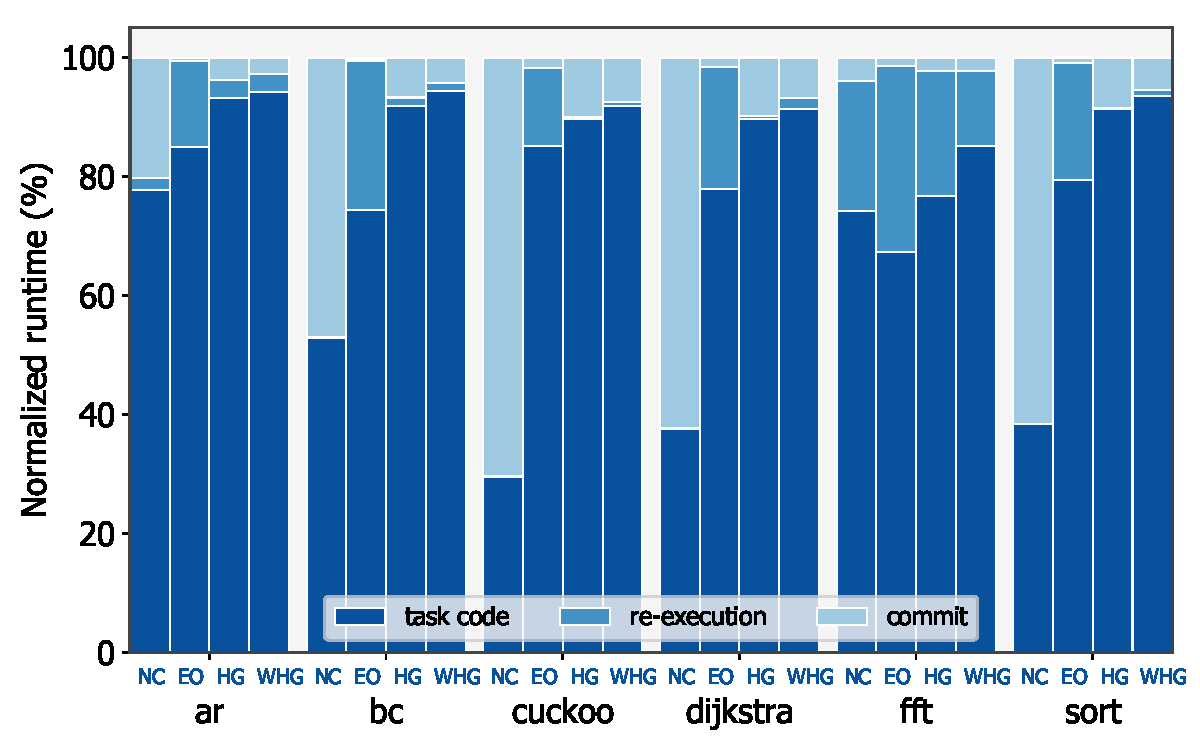
\includegraphics[width=.8\columnwidth]{figures/coalEfficiency}
    \caption{Breakdown of overhead for the proposed coalescing strategies:
    NC (no coalescing), EO (energy-oblivious), EG (energy-guided), WEG
    (weighted energy-guided). All coalescing strategies reduce total
    overhead and maximize useful work. EG and WEG perform better than EO.}
    \label{fig:overallOverheadBreakdown}
\end{figure}

For each coalescing strategy from Section~\ref{sec:task_adaptation} (EO, EG,
and WEG) and for a baseline without coalescing (NC), we have measured the time
spent on executing (i) useful task code, (ii) task code wasted due to a power failure, and
(iii) commits to non-volatile memory at the end of each (coalesced)
task.
%
The overhead incurred by each coalescing strategy is broken down in
Fig.~\ref{fig:overallOverheadBreakdown}. Without coalescing enabled (NC), the
re-execution penalty is the smallest, because the amount of work that can happen
between commits and may have to be re-executed if interrupted is reduced when
work from multiple static tasks is not combined.
%
However, any gain from a reduced re-execution penalty is canceled out by
the increased commit overhead that is incurred at the end of each static
task.
%
Across all benchmarks, will all coalescing strategies \sys reduces more commit overhead
than the re-execution overhead they add.
%
This net overhead reduction is greatest in EG and WEG strategies compared
to the EO strategy. We attribute this discrepancy to EO's slow adjustment
of the coalescing target without regard to the energy conditions.
%
In the subsequent experiments, we focus on the better-performing EG and WEG.

\paragraph{\sys's Kernel Overhead.}
%
Fig.~\ref{fig:kernel-overhead} breaks down the time spent on executing 
user task code versus the time spent on kernel operations.
When coalescing is not enabled the commit overhead is highest.
%
The overhead for memory accesses increases in percentage when enabling coalescing,
but not in absolute terms.
%
For both coalescing strategies (EG and WEG) accesses to protected variables
constitute about 30\% of the runtime overhead. Dynamic address translation
necessary on each protected access is the most critical bottleneck for \sys.

\begin{figure}
    \begin{subfigure}{\columnwidth}
			\centering
        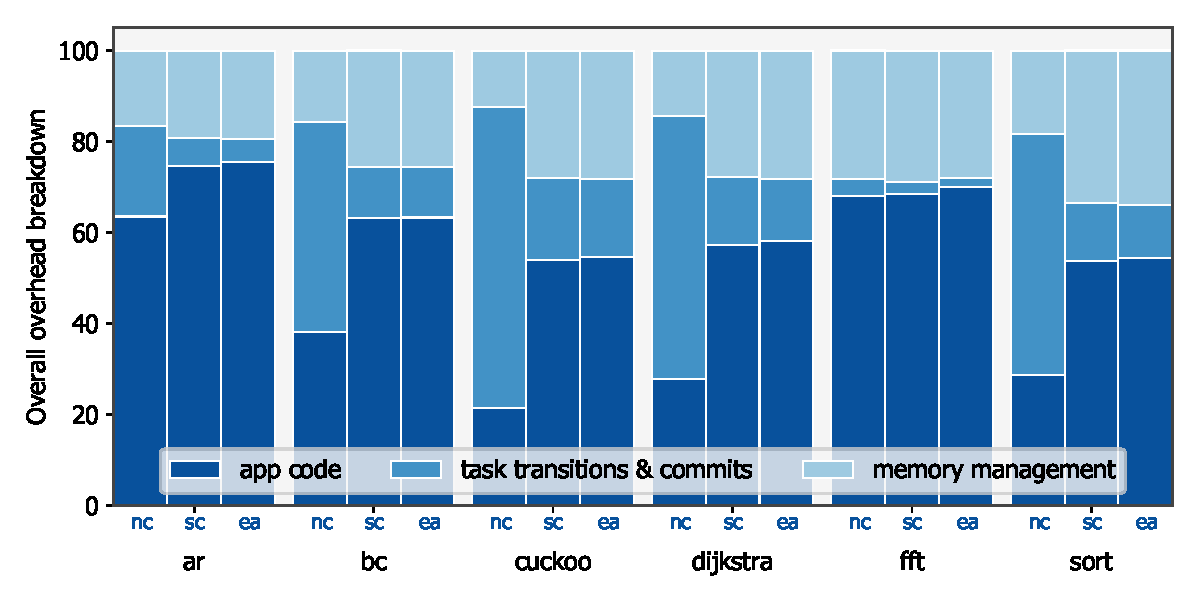
\includegraphics[width=.8\columnwidth]{figures/overallOverhead.pdf}
        \caption{Kernel overhead breakdown}
        \label{fig:kernel-overhead}
    \end{subfigure}
    \begin{subfigure}{\columnwidth}
			\centering
        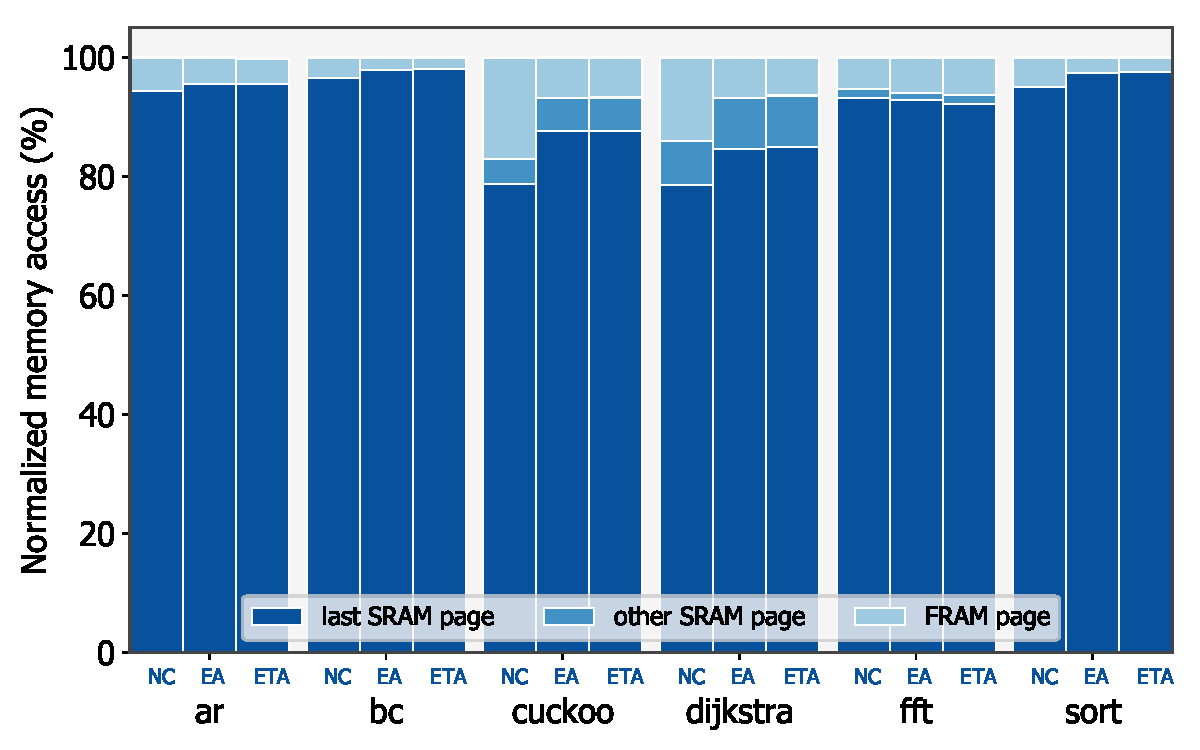
\includegraphics[width=.8\columnwidth]{figures/memAccess}
        \caption{Protected memory accesses breakdown}
        \label{fig:mem-accesses}
    \end{subfigure}
    \caption{\sys's internal overhead. NC: no coalescing, EG:
    energy-guided, WEG: weighted energy-guided.}
    \label{fig:war}
\end{figure}

\paragraph{Protected Memory Accesses Breakdown.}
%
Fig.~\ref{fig:mem-accesses} breaks down protected memory accesses
into three categories.
%
Each type of protected access incurs a different overhead.
Accessing the most recently used SRAM page is of the cheapest kind.
Accessing a different page in SRAM has a slightly higher cost.
Finally, accessing a page that needs to be swapped in
from FRAM into SRAM is the most expensive.
%
The results in the figure show that the overwhelming majority of accesses are
of the cheapest kind, which motivated us to optimize this accesses in our
implementation.
%
Only \textit{cuckoo}, \textit{dijkstra}, and \textit{fft} have non-negligible
number of accesses to a different SRAM page, which is due to the larger working
set and a less regular access pattern in these applications.
%
In general, memory access patterns are shaped by the application, and the more
program state is protected, the higher the rate of page swaps.
%
\subsection{Execution Time}
\label{sec:result_coalescing}
%
Having shown in Section~\ref{sec:coala_overhead} that coalescing reduces
overhead, we now investigate the outcome of this reduction on the total
execution time. We first investigate different variants of \sys and
then compare the best variant to Alpaca~\cite{alpaca}. Additionally, we compare \sys
performance running with different energy buffer sizes. 

\paragraph{Speedup with Coalescing.}
%
\begin{figure}
    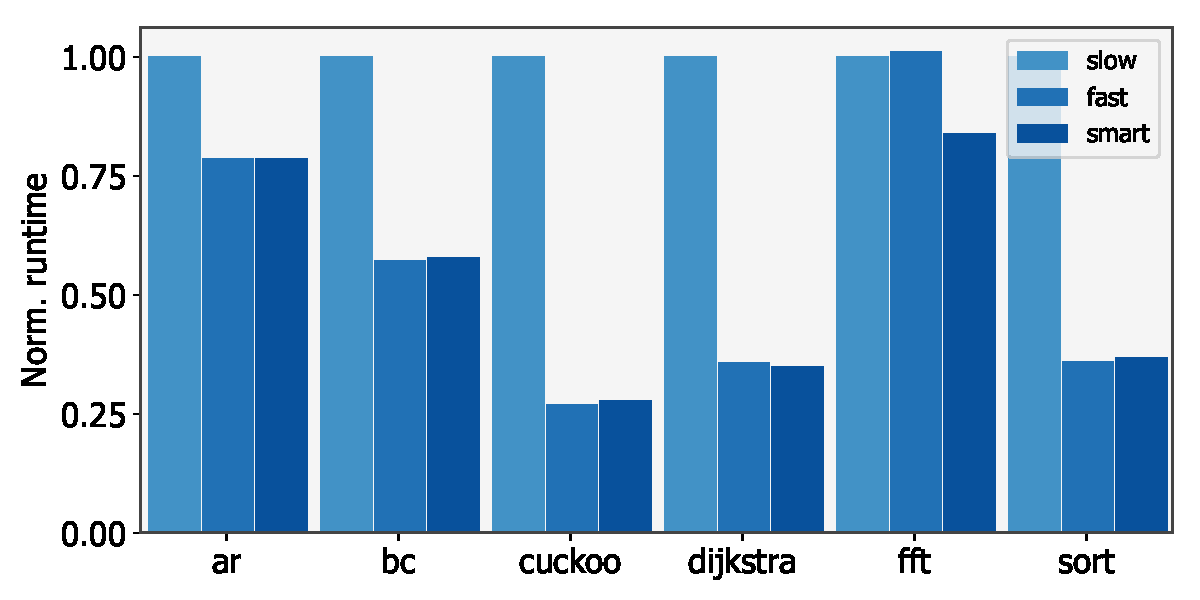
\includegraphics[width=.8\columnwidth]{figures/coalStrategies}%
    \caption{\sys's coalescing performance. Application execution time
with coalescing (EG and WEG) normalized to the execution time
without coalescing (NC).}
\label{fig:coalescing}
\end{figure}

\begin{table}
\begin{center}
\begin{tabular}{c c c c c c}
  \toprule
    \textbf{Cap. size} ($\mu\text{F}$)& \textbf{Exp. time} ($s$)& \textbf{on/off cycle} & \textbf{Coalesced task} ($ms$)   & \textbf{Runs} & \textbf{Run time} ($ms$) \\
        \hline
    47                 &1205             & 12.93\%    & 33                        & 85       & 183      \\
    470                &1205             & 12.79\%    & 88                        & 87       & 177 \\
  \bottomrule
\end{tabular}
\end{center}
\caption{Comparison of \sys performance running the \textit{sort} application on two different capacitor sizes. We see that \sys optimizes its coalesced task size based on the energy buffer size.
	\textbf{Coalesced task} refers to the first coalesced task after a reboot, \textbf{Exp. time} shows the experiment duration, the \textbf{Runs} column lists the number of complete runs of the application during the experiments. \textbf{Run time} is the device collective uptime needed to finish a single iteration of the \textit{sort} application.}
\label{tab:dif_cap}
\end{table}%

Fig.~\ref{fig:coalescing} shows \sys's run time of two coalescing
strategies (EG, WEG) normalized to the run time without coalescing (NC).
%
The results show that all benchmarks
complete faster with coalescing than without coalescing: from 25\%
(\textit{ar}) up to 70\% (\textit{sort}).
%
This speedup is a consequence of the reduced overhead demonstrated in
Section~\ref{sec:coala_overhead}.
%
However, the magnitude of the speedup is (1) highly application-dependent and
(2) largely similar across the two coalescing strategies, with the exception of
\textit{fft}.
%
In some cases (\textit{bc}, \textit{cuckoo}, \textit{sort}) WEG's task weighting
system is counter-productive.
%
This occurs in task decompositions with energy-uniform tasks, where counting
tasks disregarding their energy consumption provides an equal amount of information
with a smaller effort.
%
In \textit{fft}, tasks are not uniform, and accounting for their different weights is
beneficial. In fact, the lack of task energy awareness is detrimental: with EG
\textit{fft} runs slower than without any coalescing (NC).
%
The speedup is highest for \textit{bc}, \textit{cuckoo}, \textit{dijkstra} and
\textit{sort}, because their tasks are relatively small and are easily coalesced.
%

\begin{figure}
    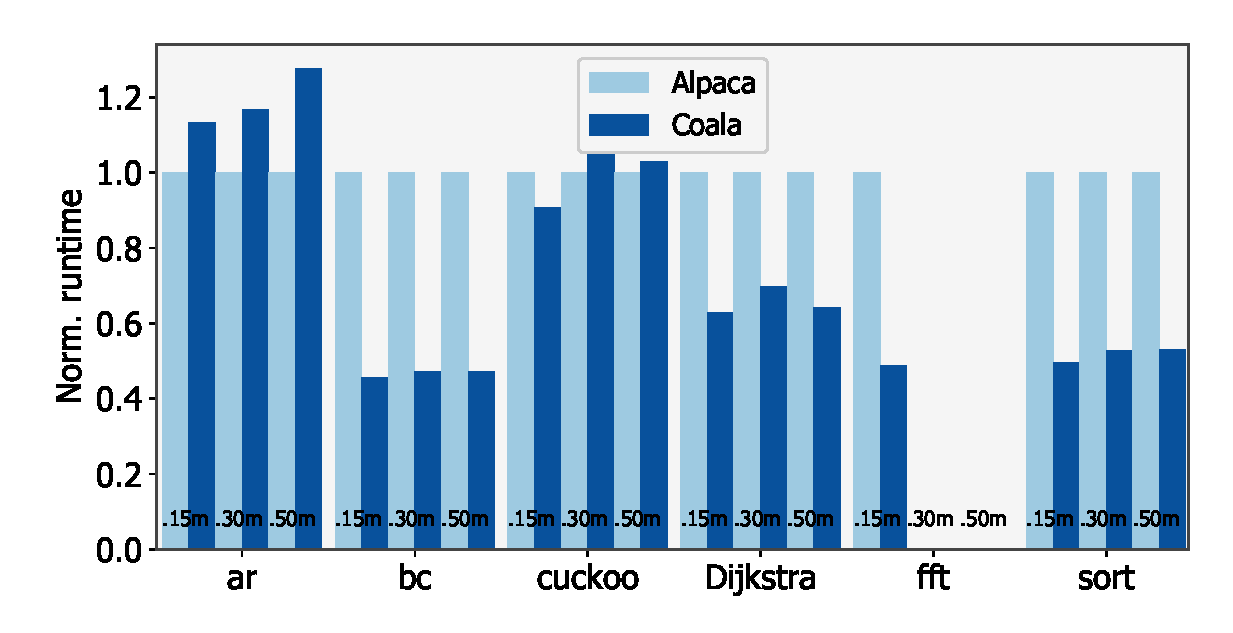
\includegraphics[width=.8\columnwidth]{figures/coala_alpaca_gcc}
    \caption{\sys's execution time normalized to Alpaca's,
    for three distances from the energy source (15, 30 and 50\,cm). }
    \label{fig:runtime}
\end{figure}

\paragraph{Benefits of Adaptive Tasks.}
%
We now compare \sys's performance to Alpaca~\cite{alpaca}---a
\emph{non-adaptive} task-based system with tasks fixed at compile-time.
Fig.~\ref{fig:runtime} shows the average execution time of each
application for \sys and Alpaca, normalized to the latter or, when not possible, to one second.
\sys provides a performance benefit compared to Alpaca for most
applications. For example, it is 54\% faster than Alpaca when executing the \textit{bc} application. In general, the speedup is greatest for applications with repeated WAR
dependencies throughout their code, particularly involving arrays
(\textit{dijkstra}, \textit{fft} and \textit{sort}). \sys's VMM
successfully amortizes the overhead of protecting memory that is accessed in
such patterns.  In applications without locality among accesses to protected
variables \sys incurs overhead from memory
virtualization that causes its performance to be comparable to (or worse than)
Alpaca (\textit{ar}, \textit{cuckoo}).

Due to its static progressing behavior, Alpaca was unable to complete the \textit{fft} benchmark on distances larger than 15\,cm\footnote{At distances less than 15\,cm the total amount of energy available for task execution includes significant amount of harvested-while-executing energy in addition to the stored energy.}.

This is marked with $\infty$ signs in Fig.~\ref{fig:runtime}. \sys, however, managed to complete \textit{fft} by enabling its task downscaling at 30\,cm and 50\,cm from the energy source.

\paragraph{Different Capacitor Sizes}
Table~\ref{tab:dif_cap} shows how \sys optimizes its Coalescing task size based on the amount of buffered energy at runtime. This means that applications implemented in \sys are portable across devices with different capacitor sizes without recompilation; they are also more resilient to degradation in capacitor size due to temperature and device lifetime. 

We see that \sys scales up its coalesced task size with a bigger energy buffer and vice versa. 
This allows it to reduce the time-to-completion of the applications. For example, 
the \textit{sort} run-time is reduced from 183\,ms to 177\,ms when the capacitor is changed from 47\,$\mu$F to 470\,$\mu$F. It should be emphasized that a device with a bigger energy buffer suffers less from power failures (but requires longer charging time). 
%However, as has been measured in Fig.~\ref{fig:overallOverheadBreakdown} and explained in Fig.~\ref{fig:coal_anatomy}, the re-execution penalty for the \textit{sort} application is negligible.  

 
Overall, \sys shows better performance than its counterpart, and it is able to overcome the \textit{big task} (i.e. \textit{fft} tasks) problem that the static task-based systems suffer from. 

\subsection{Virtual Memory Performance}
\label{sec:results_memory_management}

We characterize the performance of \sys's virtual memory sub-system in an
experiment on a continuously-powered evaluation board, as described in
Section~\ref{sec:results_hardware_software}.
% Fig.~\ref{fig:page_size} quantifies the effects of page size.

\begin{figure}
	\centering
    \begin{subfigure}{\columnwidth}
			\centering
        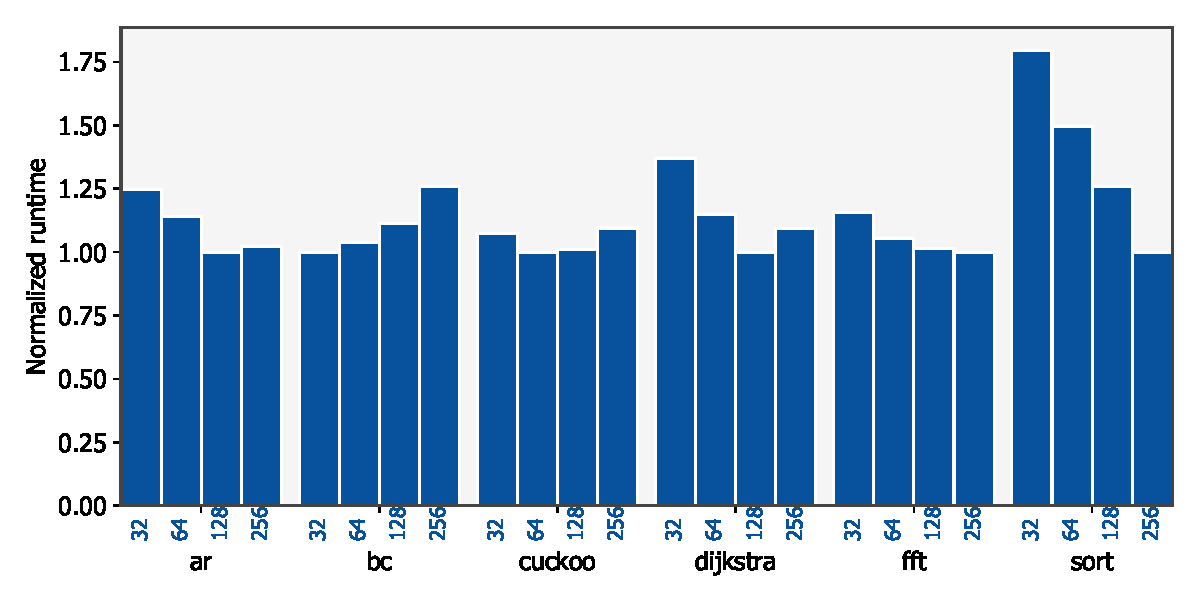
\includegraphics[width=.8\columnwidth]{figures/page_exec-time.pdf}
        \caption{Execution time normalized to lowest per-application}
        \label{fig:page-exec-time}
    \end{subfigure}
    \begin{subfigure}{\columnwidth}
			\centering
        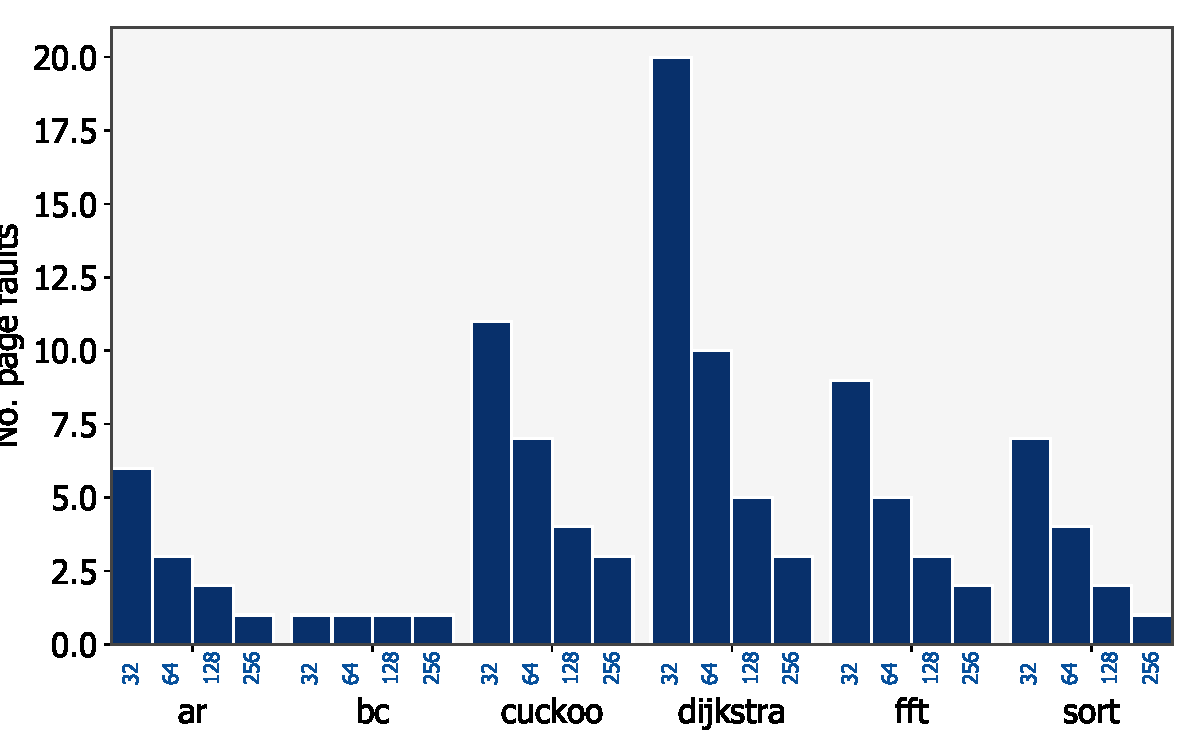
\includegraphics[width=.8\columnwidth]{figures/pagePulls.pdf}
        \caption{Number of page faults per application run}
        \label{fig:page-pulls}
    \end{subfigure}
    \caption{Effect of page size (in bytes).}
    \label{fig:war}
\end{figure}

\paragraph{Effect of Page Size on Runtime.}

Fig.~\ref{fig:page-exec-time} shows the execution time as a function
of page size (in bytes), normalized to the lowest per-application performance among the
set of page sizes.
The data suggest that there is a page size that minimizes execution time.
The best page size is not the same for
each application. Nevertheless, if a choice must be made for all applications,
128-B pages are the best option.

\paragraph{Effect of Page Size on Page Faults.}

Fig.~\ref{fig:page-pulls} reports the number of page faults, per application
run, as a function of page size (in bytes).
%
The smaller the page the more likely that a memory access will land
outside that page and that a new page will have to be swapped in.
%
This trend is visible for all applications, except for \textit{bc}. The total
amount of data accessed by \textit{bc}, as well as its working set, is small.
Even with the smallest page, all accesses are contained within that page, and
no page fault occurs. Without any page faults to begin with, increasing the
page size only yields overhead.


\section{Related Work}
\label{sec:related_work}

\textbf{Intermittently-Powered Devices.} There is a large body of research on energy harvesting and wirelessly powered embedded devices. Several recent reviews provide a broad in-depth overview~\cite{prasad_comst_2014,sample_procieee_2013,huang:commag:2015,visser_procieee_2013,kamalinejad_commag_2015,ku_cst_2016}. As computing power consumption continues to decrease, a new wave of {\em ambiently} powered systems is emerging, powered by e.g. radio waves~\cite{patel_pervasive_2017,rf_powered_computing_gollakota_2014}.
Radio-powered devices~\cite{wisp5,moo,zhao_rfid_2015,holleman_biocas_2008,thomas_jbcs_2012,naderiparizi_rfid_2015,rodriguez_tbcs_2015,liu_sigcomm_2013,kicksat,nadeau_naturebio_2017}
are related to \sys---they are the technological foundation of an
important category of intermittent computing devices. The emergence of
intermittent computing hardware platforms has led to the development of tooling
and instrumentation for such systems building~\cite{hester_sensys_2014,hester_sensys_2015,edb,stork,wisent}.

\textbf{Intermittent Execution Environments.} Early work on energy-harvesting runtime systems assumed simple, small computations not exceeding a predictable burst of energy~\cite{dewdrop} or long power-cycles/priority-based scheduling~\cite{sorber_sensys_2007}. These efforts did not consider data consistency with intermittence. Works supporting intermittent computing using dynamic, on-demand checkpoints include Mementos~\cite{mementos}, Quickrecall~\cite{quickrecall}, Hibernus++~\cite{hibernusplusplus} and HarvOS~\cite{mottola2017harvos}. Dynamic checkpointing systems may checkpoint
at any point, making it difficult to implement application-level atomicity
requirements. Moreover, some require hardware to measure stored energy, incurring energy cost. Moreover, these systems do not checkpoint non-volatile state, compromising memory consistency. DINO~\cite{dino} selectively versions non-volatile memory and checkpoints volatile state, ensuring progress and memory consistency. Rachet~\cite{ratchet} assumes all memory is non-volatile and checkpoints volatile state. Clang~\cite{hicks_isca_2017} takes a Ratchet-like approach leveraging special hardware, eliminating checkpointing and versioning overhead. 

Recent task-based systems are Chain~\cite{chain} and Alpaca~\cite{alpaca}. Using static tasks, they eliminate checkpointing volatile state. Using channel-based memory models~\cite{chain} or automatic privatization and redo-logging~\cite{alpaca} they avoid checkpointing overheads. Moreover, task-based models facilitate specifying application-level atomicity properties.

\sys relates to the above efforts but is distinct in approach and mechanism. \sys relates closely to task-based models because \sys also relies on statically defined tasks to avoid checkpointing volatile state. \sys's automatic compilation spares the programmer's work of writing task-based code that prior systems demand. \sys's memory virtualization provides an alternative for ensuring memory consistency, optimized for bulk accesses to task-shared data with high locality. \sys's task coalescing optimization ameliorates the key overheads associated with prior systems.

One approach to decrease the task count, without assuming a minimum level of
incoming power always available, is to predict task energy consumption and
choose a decomposition specific to the device capacitor size~\cite{cleancut}.
However, statically predicting energy of arbitrary input-dependent code with
peripheral access is a problem without a general solution. Furthermore, a
static decomposition approach prevents portability across devices with
different storage capacitors.

\textcolor{red}{TODO: make this one paragraph with the CleanCut stuff.  add \cite{intel} work; separate by-programmer and by-compiler;
both cases hit the energy estimation problem; also intel work proposes a method
for decomposing into one of many decompositions, but does not give a good
solution for choosing one} 



\textbf{Memory Virtualization.} Prior work on embedded systems has studied a variety of memory virtualization strategies relating to \sys. TinyOS~\cite{levis2005tinyos} and nesC~\cite{nesc} support dynamic memory management. Later work extended the memory manager to support memory virtualization backed by flash memory~\cite{sensornetvm} and to ensure memory and type safety~\cite{tinyosmemorysafety}. SOS~\cite{sos}, Contiki~\cite{contiki}, and
t-kernel~\cite{tkernel} also developed memory management abstractions that
virtualize memory size and provide safe and indirect access. Mat\'e~\cite{mate} developed full virtual machines support for sensor nodes, virtualizing not just memory resources, but other states and peripherals. The goal of \sys is to provide consistent, intermittent execution, leveraging the benefits of efficient bulk copying. In contrast, prior efforts focused more on programmability and runtime reliability properties provided by virtual memory.

Another \sys-related prior effort is on unbounded, page-based transactional memory and deterministic parallel runtime systems~\cite{pagebasedtm,grace}. These works have a different mechanism and purpose than \sys---ensuring that data are consistent and deterministically updated during concurrent executions. What makes these
efforts related is that they manage state to ensure consistency at the
granularity of pages to amortize checking and tracking costs. \sys also tracks
accesses at the granularity of a page and uses its paging mechanism to ensure
consistency. Moreover, \sys's paging implementation, which keeps a shadow page
for each page to use during commit, is similar to the shadow paging scheme
use for transactional commit~\cite{pagebasedtm}.


\section{Conclusions}
\label{sec:conclusions}

This paper presented \sys: a new task-based runtime for intermittently-powered devices that does not require any hardware support. \sys core new features are: (i) automatic task-generation---removing programmer intervention in the program re-composition to the intermittent domain \emph{completely}, (ii) memory virtualization---reducing the execution speeds by \todo{provide numbers}{Przemek} of broad set of benchmarks executed on popular energy-harvesting embedded platform, and (iii) (adaptive) task coalescing---enabling fastest execution \todo{provide numbers}{Przemek} despite changing energy arrivals and enabling re-use of the same code on intermittent systems with varying energy reservoirs. \sys, with its task creation/execution automation, responses to the need that all existing predecessors of \sys (chronologically, Mementos, DINO, Chain, Alpaca) strongly advocated. We believe that \sys is a next major step in enabling computing community to enter the intermittent-power domain without big learning curve investments. Next logical step in \sys design is the introduction of features needed to implement first fully-operational operating system for transiently-powered devices.\todo{find a more convincing reason for a follow-up work}{Brandon} \todo{Revise this section}{Brandon}

\bibliographystyle{ACM-Reference-Format}
%\bibliographystyle{plain}
\bibliography{bib}

\end{document}
